%
% Tesi D.S.I. - modello preso da
% Stanford University PhD thesis style -- modifications to the report style
%
%%%%%%%%%%%%%%%%%%%%%%%%%%%%%%%%%%%%%%%%%%%%%%%%%%%%%%%%%%%%%%%%%%%%%%%%%%%
%                                                                         %
%			TESI DOTTORATO                                                   %
%			______________                                                   %
%                                                                         %
%			AUTORE: Elena Pagani                                             %
%                                                                         %
%			Ultima revisione: 7.X.1998                                       %
%           correzioni atrent                                             %
%%%%%%%%%%%%%%%%%%%%%%%%%%%%%%%%%%%%%%%%%%%%%%%%%%%%%%%%%%%%%%%%%%%%%%%%%%%
%
%
\documentclass[a4paper,12pt]{report}
%    \renewcommand{\baselinestretch}{1.6}      % interline spacing
%
% \includeonly{}
%
%			PREAMBOLO
%
\usepackage[a4paper]{geometry}
\usepackage{amssymb,amsmath,amsthm}
\usepackage{graphicx}
\usepackage{url}
\usepackage{hyperref}
\usepackage{epsfig}
\usepackage[italian]{babel}
\usepackage{setspace}
\usepackage{packages/tesi}
\usepackage{xcolor}
\usepackage[ruled, italiano, linesnumbered]{packages/algorithm2e}
\usepackage{booktabs}
\usepackage{siunitx}
\usepackage{float}
\usepackage{tabularx}
\sisetup{output-decimal-marker={.}}
\newcommand{\expnumber}[2]{{#1}\mathrm{e}{#2}}
\def\HiLi{\leavevmode\rlap{\hbox to \hsize{\color{yellow!50}\leaders\hrule height .8\baselineskip depth .5ex\hfill}}}
% per le accentate
\usepackage[utf8]{inputenc}
%
\newtheorem{myteor}{Teorema}[section]
%
\newenvironment{teor}{\begin{myteor}\sl}{\end{myteor}}
%
%
%			TITOLO
%
\begin{document}
\title{Temp Identificazione di Satelliti}
\author{Jonathan Junior AGYEKUM}
\dept{Corso di Laurea in Informatica}
\anno{2022-2023}
\matricola{935132}
\relatore{Prof. Giovanni RIGHINI}
%
%        \submitdate{month year in which submitted to GPO}
%		- date LaTeX'd if omitted
%	\copyrightyear{year degree conferred (next year if submitted in Dec.)}
%		- year LaTeX'd (or next year, in December) if omitted
%	\copyrighttrue or \copyrightfalse
%		- produce or don't produce a copyright page (false by default)
%	\figurespagetrue or \figurespagefalse
%		- produce or don't produce a List of Figures page
%		  (false by default)
%	\tablespagetrue or \tablespagefalse
%		- produce or don't produce a List of Tables page
%		  (false by default)
%
%			DEDICA
%
\beforepreface
\prefacesection{}
        {\hfill \Large {\sl dedicato a \dots}}
%
%			PREFAZIONE
%
\prefacesection{Prefazione}
prefazione
%
%
%			ORGANIZZAZIONE
\section*{Organizzazione della tesi}
\label{organizzazione}
La tesi \`e organizzata come segue:
\begin{itemize}
\item nel Capitolo 1 ....
\end{itemize}
%
%			RINGRAZIAMENTI
%
\prefacesection{Ringraziamenti}
Grazie.
\afterpreface
%
%
%			CAPITOLO 1: Introduzione
\chapter{Introduzione}
\label{cap1}
\section{Strumenti utilizzati}
\section{Ricerca operativa e astronomia}
\section{Storia dell'identificazione di satelliti}
\subsection{Rilevamenti diretti e indiretti}

%
%
%			CAPITOLO 2: Descrizione del problema
\chapter{Descrizione del problema}
\label{cap2}
\section{Descrizione}
L'osservazione in modo continuo dell'angolo descritto da  k~satelliti intorno al loro pianeta, genera delle sinusoidi, questo apre alla possibilità di una identificazione dei satelliti attraverso l'analisi del loro moto orbitale.

Il legame tra l'orbite dei satelliti e le sinusoidi può essere spiegata considerando le orbite dei satelliti circolari e quindi attraverso le leggi del moto circolare.
\begin{figure}[H]
  \caption{Moto circolare uniforme}
  \begin{center}
  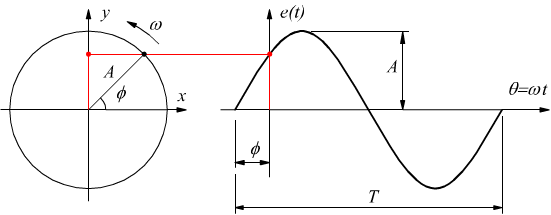
\includegraphics[scale=0.50]{img/sinusoide_cerchio.png}
  \begin{tabular}{r@{: }l r@{: }l}
  $T$ & Periodo & $\phi$ & Fase \\
  $A$ & Ampiezza & $\omega$ & Velocità angolare
  \end{tabular}
  \end{center}
\end{figure}

% spiegare meglio relazione

Dove il periodo corrisponde al tempo di rivoluzione del satellite, l'ampiezza alla massima distanza che intercorre nel periodo tra il satellite e il corrispettivo pianeta, e(t) lo spostamento del satellite lungo l'orbita. È quindi possibile descrivere la sinusoide risultante tramite l'espressione analitica:
$ e(t) = A\sin(\omega t + \phi)$



L'obiettivo è quello di riuscire ad attribuire ai k satelliti i k valori di
ogni osservazione e di trovare periodo, ampiezza e fase delle k sinusoidi,
supponendo di poter osservare i k valori simultaneamente, in n momenti
successivi. Si suppone di non conoscere nulla dei k satelliti e sopratutto di non poterli distinguere in fase di rilevazione dei valori.

Il problema è scomponibile in due sottoproblemi: uno di interpolazione e uno di assegnamento. La componente di interpolazione è identificata nell'operazione di individuazione della sinusoide che si scosta il meno possibile dai valori. Questo definisce un problema di interpolazione non-lineare e continuo: non-lineare poiché una sinusoide è una funzione periodica non-lineare, definita da una trasformazione elementare della funzione seno, continuo poiché il dominio di una sinusoide e delle sue componenti è definito in $\mathbb{R}$ o in un suo sottoinsieme.

La componente di assegnamento è individuata nel processo di selezione dei punti tra le diverse osservazioni da interpolare.
La funzione di questa componente è quella di individuare k sinusoidi, generate dall'interpolazione di una assegnazione di valori, che rappresentino i k satelliti.



\section{Campi di applicazione e utilità}
Il principio della tipologia di identificazione che ho studiato è quello di riconoscere satelliti di un pianeta in base alla variazione in un determinato dominio di una caratteristica quantificabile, in questo caso l'angolo, in funzione del tempo. La variazione dev'essere riconoscibile e identificativa del satellite, cioè deve definire un andamento caratteristico di una funzione elementare o una combinazione di essi. Questo principio è illustrato, per esempio dal metodo di trasito, metodo di identificazione fotometrico di satelliti extrasolari \cite{transito}.

La tipologia di identificazione che illustrerò, può essere applicata sia ai casi di rilevamento diretto, tecniche che permettono di osservare direttamente al telescopio i satelliti, e sia indiretti, cioè l'individuazione tramite effetti fisici che satellite può indurre. Il vincolo fondamentale è che sia possibile effettuare misurazioni dell'angolo rispetto al suo pianeta.

L'identificazione attraverso l'analisi del moto orbitale può essere utile in tutte le situazioni dove non è possibile riconoscere o distinguere due o più satelliti o qualunque entità il quale movimento è osservabile e rotante.





%
%
%			CAPITOLO 3: Sviluppo del modello
\chapter{Sviluppo del modello}
\section{Definizione del modello}
% l'interpolazione ha due obiettivi max periodo e min errore
Propongo un modello per la risoluzione del sottoproblema di interpolazione.
La sinusoide che si vuole ottenere dall'interpolazione dei punti deve avere determinate caratteristiche. Tra tutte le sinusoidi possibili che interpolano gli n valori, che in questo contesto chiamerò punti, si vuole quella di massimo periodo e sicché le misurazioni possono essere affette da errore si deve combinare la ricerca del massimo periodo con quella di minimo errore, definendo un problema a due obiettivi.

Il processo risolutivo per un problema a molti obiettivi in conflitto tra loro, cioè che il miglioramento di una comporti un peggioramento di un'altra, prevede:
\begin{enumerate}
  \item Il calcolo della regione pareto-ottima, cioè l'insieme di soluzioni ammissibili non dominate, denominate anche soluzioni paretiane.
  \item La scelta di una soluzione tra quelle individuate.
\end{enumerate}
La determinazione della regione pareto-ottima può essere effettuata in diversi modi. I modelli che ho definito inseguito utilizzano rispettivamente metodo dei pesi e metodo dei vincoli, i due modelli si differenziano solo per vincoli e funzione obiettivo.

In questo processo di interpolazione è necessario fare attenzione alle sinusoidi con basso periodo rispetto alla sinusoide da individuare: si può osservare dalle regioni paretiane rappresentate dalle figure da \ref{fig:reg_ammis_10_0010} a \ref{fig:reg_ammis_30_0010} del paragrafo \ref{ss:sel_sol} che aumentando la frequenza, quindi al diminuire del periodo, esiste sempre un modo di interpolare n punti con una sinusoide minimizzando a piacimento l'errore di interpolazione.

% perché
% dati
\paragraph{Parametri}

I dati a disposizione del modello sono gli n punti assegnati da interpolare, il quale numero è determinato dal modulo di assegnamento. I punti sono individuati in un piano cartesiano dove l'asse delle ascisse rappresenta il tempo e l'asse delle ordinate l'angolo. I parametri del modello sono quindi le n ascisse $t_i$ e le n ordinate $e_i$ degli n punti, con $i$ da 1 a n.

Per una maggiore semplicità numerica considero i secondi per il tempo mentre rappresento gli angoli in radianti.


% variabili
\paragraph{Variabili}
Le variabili sono individuate nelle componenti che determinano una sinusoide, data l'espressione analitica generale di una funzione sinusoidale:
\begin{equation}
e_i = A\sin(\omega t_i + \phi)
\end{equation}

Dall'espressione ho definito le variabili che rappresentano fase $ \phi $, ampiezza $ A $  e la pulsazione $\omega$.

Inoltre c'è la necessità di rappresentare l'errore che può essere generato dalle misurazioni o da un assegnamento di punti errato. L'espressione analitica diventa:
\begin{equation}
\label{vin:sin}
e_i = A\sin(\omega t_i + \phi) + \varepsilon_i
\end{equation}

Perciò ho definito n variabili aggiuntive che rappresentano l'errore per ogni punto.
\subsection{Calcolo della regione pareto-ottima}

\subsubsection{Metodo dei pesi}
Il metodo dei pesi consiste nel dare un peso a ciascuna delle funzioni obiettivo, così da ridurre il problema a molti obiettivi in uno di programmazione matematica parametrica.

\subparagraph{Vincoli}
Ho definito come unico vincolo l'equazione~\eqref{vin:sin}

\subparagraph{Funzione obiettivo}
Le due funzioni obiettivo da ottimizzare sono:

\begin{equation}
\label{fo:periodo}
min \, f_1 = \omega
\end{equation}
La massimizzazione del periodo
\begin{equation}
\label{fo:errore}
min \, f_2 = \sum_{i=1}^n \varepsilon_i^2
\end{equation}
La minimizzazione dell'errore complessivo, calcolo l'errore qudratico complessivo per l'eliminazione dei possibili valori negativi che si possono generare.

I pesi definiti per le funzioni $ f_1 $ e $ f_2 $ sono rispettivamente 1 e -1, quindi ottenendo la funzione obiettivo:

\begin{equation}
max \, f = f_1 + f_2
\end{equation}
Questa configurazione dei pesi di partenza permette di penalizzare tutte quelle soluzioni ammissibili che massimizzano il periodo ma hanno un errore elevato.

Il processo di individuazione delle soluzioni paretiane, con questo metodo e numero di funzioni, consiste nel eseguire un analisi parametrica sui pesi, cioè analizzare e individuare soluzioni non dominate al variare dei pesi entro un certo range. In questo caso può essere sufficiente solo effettuare la variazione del peso dell'errore.

Un modello che da priorità al periodo ottenendo un alto errore è per certo non utilizzabile, perché l'alto errore denota una completa mancanza di relazione tra i punti e la sinusoide individuata, questo spiega l'analisi parametrica solo sul peso dell'errore. È anche possibile non è effettuare alcuna variazione dei pesi, ed accontentarsi della prima soluzione individuata tramite la configurazione dei pesi di partenza.

\subsubsection{Metodo dei vincoli}
Il metodo dei vincoli consiste nell'ottimizzare una delle funzioni obiettivo, trasformando le rimanenti in vincoli, utilizzando un termine noto parametrico.

\subparagraph{Vincoli} Si ha l'equazione~\eqref{vin:sin} e la trasformazione in vincolo della funzione obiettivo legato al periodo~\eqref{fo:periodo}
\begin{equation}
\label{vin:periodo}
\frac{2\pi}{\omega} \ge \beta
\end{equation}
Il termine noto $ \beta $ sta ad indicare il minimo periodo ammissibile per una soluzione, questo permette di escudere le soluzioni a basso periodo rendendo inammisibili soluzioni con periodo più piccolo del termine noto.

\subparagraph{Funzione obiettivo}
La funzione obiettivo definita è la funzione \eqref{fo:errore}.

L'individuazione delle soluzioni paretiane è effettuata variando il termine noto parametrico nel vincolo \eqref{vin:periodo}.
Ho scelto di definire il vincolo \eqref{vin:periodo} perché permette di avere un controllo migliore sull'esplorazione dei periodi possibili della sinusoide da individuare, data dalla possibilità di definire come punto di partenza del modello, un assegnazione della variabile che rappresenta la pulsazione a partire dal termine noto~$\beta $.
\begin{equation}
  \omega = \frac{2\pi}{\beta}
\end{equation}
Da un analisi ipotetica dei range di periodi, che possono essere rilevati nel campo di applicazione in questione, è possibile esplorare e individuare sinusoidi entro il range ipotizzato. Al contrario definendo un vincolo a partire dalla funzione obiettivo dell'errore \eqref{fo:errore}, sarebbe di difficile gestione e modellazione la determinazione della variazione dell'errore, per tutte le tipologie di assegnamenti di punti della quale può essere richiesta l'interpolazione ad esempio: punti completamente non relazionati tra di essi, punti rilevati con un alto errore nel processo di misurazione.


\section{Algoritmo di controllo}
\label{ss:controllo}
% scelta del modello da utilizzare
Il modello che ho scelto di implementare è il modello che utilizza il metodo dei vincoli per i vantaggi citati nella sua specificicazione. Una volta definito l'implementazione del modello è necessario specificare un algoritmo di controllo e di esecuzione di esso. I compiti sono la definizione del valore del minimo periodo $ \beta $, nel vincolo \eqref{vin:periodo} ad ogni iterazione e la gestione di eventuali errori.

\begin{algorithm}
  \caption{Algoritmo di controllo del modello}
  \label{controllo}
  \SetKwInOut{Input}{input}\SetKwInOut{Output}{output}
  \SetKwData{Pt}{pt}
  \SetKwData{Soluzioni}{soluzioni}
  \SetKwData{Passo}{passo}
  \SetKwData{Sol}{sol}
  \SetKwData{SolPrecedente}{solPrecedente}
  \SetKwFunction{Interpola}{Interpola}
  \SetKwFunction{F}{f}

  \BlankLine
  \Input{\Pt Collezione di punti da interpolare $[(t_1, e_1), ..., (t_k, e_k)]$}
  \Output{\Soluzioni Insieme di soluzioni che interpolano i punti $pt$}
  \BlankLine

  \Passo $\leftarrow 1$ \\
  $\beta \leftarrow periodoIniziale$ \\
  \Soluzioni $\leftarrow \emptyset$ \\
  \While{$\beta <= periodo Limite$}{ \label{periodoLimite}
      \SolPrecedente $\leftarrow$ \Sol \\
      \Sol $\leftarrow$ \Interpola{\Pt, $\beta$, solutore} \\ \label{interpola}
      Aggiungi \Sol a \Soluzioni \\
      \eIf{$\Sol[periodo] = \SolPrecedente[periodo]$}{ \label{aumentoPasso}
      \Passo = \F{\Passo} \\ \label{velocitaPasso}
      }{
      \Passo $\leftarrow 1$ \\ \label{passoDefault}
      }
      $\beta \leftarrow \beta + \Passo$ \\

  }


\end{algorithm}

% Metodo di esplorazione del range
\subsection{Definizione del passo per il minimo periodo $\beta$}
\label{ss:passo}
Il passo definisce la quantità aggiunta al minimo periodo ad ogni iterazione.
Per facilitare l'individuazione di soluzioni differenti, è possibile definire un passo variabile, così da spostare il punto di inizializzazione del problema dalla regione di un minimo locale, in base alla soluzione ottenuta.



L'algoritmo va ad aumentare il passo ogniqualvolta il periodo della soluzione individuata in una iterazione, appartiene ad un intorno del periodo della soluzione dell'iterazione precedente (riga \ref{aumentoPasso}), altrimenti si ha un ripristino del passo ad un valore di default (riga \ref{passoDefault}). In base alle necessità è possibile definire velocità differenti di variazione del passo, tramite la definizione della funzione $f$ (riga \ref{velocitaPasso}). Per aumentare il numero di soluzioni individuate è necessario diminuire la velocità di variazione di passo in modo da ottenere inizialmente piccoli spostamenti del minimo periodo, al contrario per ottenere meno soluzioni ed una esplorazione più veloce, è necessario aumentare la velocità di variazione del passo. esempi possono essere:
\begin{equation}
  \label{velocitaPassoEspl}
f(x) = x * k
\end{equation}
Si moltiplica il passo p per una costante k, è possibile variare la velocità della variazione del passo aumentando o diminuendo il parametro k. Si misura la velocità della funzione di variazione del passo tramite la derivata della funzione $f(x)$.

Un altro fattore che determina l'esplorazione è la dimensione dell'intorno. È necessario definire un intorno poiché è possibile che con approssimazioni e specifiche interne del solutore o anche in base alle caratteristiche della regione ammissibile, non si individui l'esatto valore di un minimo locale, ma un valore nell'intorno di esso in iterazioni successive. Perciò è necessario definire un livello di tolleranza con il quale definire se due soluzioni sono da cosiderare uguali (riga \ref{aumentoPasso}).
% definizione del range di periodi

\subsection{Punto di inizializzazione}
Il processo di inzializzazione di un modello, consiste nel fissare le variabili del problema a dei valori di partenza. Generalmente definire una soluzione iniziale per il solutore nei problemi di programmazione non lineare è importante, poiché ne determina l'abilità di individuare un minimo locale diverso da un altro, e poter indidivuare un minimo locale migliore sotto una determinata caratteristica.

In questo problema la qualità della soluzione è individuata prevalentemente nel periodo e nell'errore, perciò la variabile che assume più importanza nella determinazione di una soluzione iniziale è la pulsazione $\omega$, gli errori per ogni punto sono variabili risultanti perciò non vanno fissate.

Con questa definizione del modello, mi è risultato difficile discernere un algoritmo di definizione della soluzione di partenza, a partire dai test effettuati. La difficoltà nasce dal interpretare il comportamento del solutore dato un problema e una serie di soluzioni di partenza all'aumentare del minimo periodo $ \beta $, quindi dall'indiviuazione di un pattern chiaro e veloce che definisca la posizione ideale della soluzione di partenza, nelle successive iterazioni.

I test sono stati effetuati eseguendo l'algoritmo di controllo, \ref{controllo} dando come punto di iniziale il seguente:
\begin{itemize}
  \item $A$ = 0
  \item $\phi$ = 0
  \item $w = \frac{4\pi}{5000 - \beta}$
\end{itemize}

Con i seguenti parametri dell'algoritmo \ref{controllo}:
\begin{itemize}
  \item $f(x)$ in riga \ref{velocitaPasso}, algoritmo \ref{controllo} pari alla funzione \eqref{velocitaPassoEspl} con $k = 5$
  \item $periodoIniziale = 0s$
  \item $periodoFinale = 5000s$
\end{itemize}

Fissando $ \omega $ con il periodo a metà tra il periodo limite e il minimo periodo $\beta$, ad esempio nel problema con 30 punti generati dalla sinusoide $ e(t)~=~sin(\omega t)$

\begin{table}[H]
  \caption{Iterazioni effettuate per il problema con Sinusoide con $\omega = 0.8~rad/s$}
  \label{tab:init_08}
  \begin{center}
    \begin{tabularx}{\textwidth}{SSSp{0.5\textwidth}}
      \toprule
      {Periodo limite $\beta$ (s)} & {Periodo di partenza (s)} & {Periodo soluzione (s)} & {Errore quadratico \newline medio} \\
      \midrule
      1 &  1201 & 7.5 & $\expnumber{1.3}{-11}$\\
      2 &  2095 & 10.3 & $\expnumber{7.5}{-5}$\\
      7 &  4175 & 10.9 & $\expnumber{3.2}{-4}$\\
      32 &  4175 & 10.9 & $\expnumber{3.2}{-4}$\\
      157 &  4175 & 10.9 & $\expnumber{3.2}{-4}$\\
      782 &  4175 & 10.9 & $\expnumber{3.2}{-4}$\\
      3907 &  4175 & 10.9 & $\expnumber{3.2}{-4}$\\
      4532 &  4175 & 10.9 & $\expnumber{3.2}{-4}$\\
      4657 &  4175 & 10.9 & $\expnumber{3.2}{-4}$\\
      \bottomrule
    \end{tabularx}
  \end{center}
\end{table}


\subsection{Criterio arresto }
\label{ss:arresto}
È necessario specificare un criterio di arresto per l'algoritmo di controllo. L'idea applicata è quella di determinare l'arresto fissando un periodo limite per il minimo periodo $ \beta $ (riga \ref{periodoLimite}). Effettuando una ricerca sui satelliti del sistema solare, ho individuato che il massimo periodo di un satellite nel sistema solare è pari a 9374.0 giorni \cite{nasa}.

Quindi è possibile fissare un periodo limite, effettuando un mappaggio da giorni in secondi, pari a 5000s.
Non è necessario fissare esattamente il valore estratto dallo studio dei periodi del sistema solare, poiché il periodo $ \beta $, utilizzato nel vincolo \eqref{vin:periodo}  come limite inferiore, non impedisce al solutore di individuare periodi dai valori molto più grandi rispetto ai periodi del sistema solare, tutto questo facendo partire l'individuazione delle soluzioni da un periodo pari a 0, escudendo i periodi negativi. L'esclusione dei periodi negativi non influisce sull'individuazione delle soluzioni poiché i punti sono rilevati all'avanzare del tempo.

% scelta del solutore da utilizzare
\subsection{Scelta del solutore}
\label{ss:scelta_solutore}
A causa dei vincoli di utilizzo dei solutori globali in nlopt \cite{nlopt}, la scelta del solutore è ricaduta ai solutori locali (riga \ref{interpola}). È possibile condurre la selezione dell'algoritmo solutore valutandoli su problemi di interpolazione definiti da punti appartenenti ad una stessa sinusoide $ e(t)~=~sin(\omega t)$ per un numero di punti definito. Le ascisse dei n punti assumono i valori interi dell'insieme [0, n]. Analizzo il numero totale di soluzioni individuate, il numero di soluzioni individuate in un intorno del periodo della sinusoide del problema, infine il tempo di calcolo.
L'intorno scelto è di dimensioni pari a 100s, è possibile scegliere un diverso intorno in base alle proprie necessità di precisione rispetto alla sinusoide da individuare.

I risultati delle sperimentazioni sono illustrati nelle tabelle da \ref{tab:prestazioni_sol8} a \ref{tab:prestazioni_sol0010}.
I parametri dell'algoritmo \ref{controllo} per le seguenti sperimentazioni sono:
\begin{itemize}
  \item $f(x)$ in riga \ref{velocitaPasso}, algoritmo \ref{controllo} pari alla funzione \eqref{velocitaPassoEspl} con $k = 2$
  \item $periodoIniziale = 0s$
  \item $periodoFinale = 5000s$
\end{itemize}

\begin{table}[H]
  \caption{Prestazioni dei solutori: Sinusoide con $\omega = 0.8~rad/s$}
  \label{tab:prestazioni_sol8}
  \center
    \begin{tabular}{lSSS}
      \toprule
      {Solutore} & {n. soluzioni individuate} & {n. soluzioni nell'intorno} & {Tempo di calcolo (s)} \\
      \midrule
      COBYLA & 120 & 21 & 6.1 \\
      BOBYQA & 19   &     6     &  0.9   \\
      NEWUOA & 113  &    101    &  5.9 \\
      PRAXIS & 139  &    139    &  6.9 \\
      SBPLX  & 26    &     9    &  1.3 \\
      \bottomrule
    \end{tabular}
\end{table}

\begin{table}[H]
  \caption{Prestazioni dei solutori: Sinusoide con $\omega = 0.0125~rad/s$}
  \label{tab:prestazioni_sol0125}
  \center
    \begin{tabular}{lSSS}
      \toprule
      {Solutore} & {n. soluzioni individuate} & {n. soluzioni nell'intorno} & {Tempo di calcolo (s)} \\
      \midrule
      COBYLA & 141  &    19     &  7.1 \\
      BOBYQA & 20   &     0     &   1.0 \\
      NEWUOA & 114   &     0    &   5.7 \\
      PRAXIS & 139   &     0     &  6.9 \\
      SBPLX  & 26   &     1     &   1.3 \\
      \bottomrule
    \end{tabular}
\end{table}

\begin{table}
  \caption{Prestazioni dei solutori: Sinusoide con $\omega = 0.005~rad/s$}
  \label{tab:prestazioni_sol005}
  \center
    \begin{tabular}{lSSS}
      \toprule
      {Solutore} & {n. soluzioni individuate} & {n. soluzioni nell'intorno} & {Tempo di calcolo (s)} \\
      \midrule
      COBYLA & 218  &     3     &  11.0 \\
      BOBYQA & 20   &     0     &   1.0 \\
      NEWUOA & 113  &     0     &   5.6 \\
      PRAXIS & 149  &     0     &  7.4 \\
      SBPLX & 25   &     0     &   1.2 \\
      \bottomrule
    \end{tabular}
\end{table}

\begin{table}[H]
  \caption{Prestazioni dei solutori: Sinusoide con $\omega = 0.0013~rad/s$}
  \label{tab:prestazioni_sol0013}
  \center
    \begin{tabular}{lSSS}
      \toprule
      {Solutore} & {n. soluzioni individuate} & {n. soluzioni nell'intorno} & {Tempo di calcolo (s)} \\
      \midrule
      COBYLA & 193  &     4     &  9.8 \\
      BOBYQA & 19   &     0     &  0.9 \\
      NEWUOA & 113   &     0    &  5.6 \\
      PRAXIS & 146   &     0    &  7.3 \\
      SBPLX  & 24   &     0     &  1.2 \\
      \bottomrule
    \end{tabular}
\end{table}

\begin{table}[H]
  \caption{Prestazioni dei solutori: Sinusoide con $\omega = 0.0010~rad/s$}
  \label{tab:prestazioni_sol0010}
  \center
    \begin{tabular}{lSSS}
      \toprule
      {Solutore} & {n. soluzioni individuate} & {n. soluzioni nell'intorno} & {Tempo di calcolo (s)} \\
      \midrule
      COBYLA & 54   &    0      &  2.7 \\
      BOBYQA & 19   &    0      &  0.9 \\
      NEWUOA & 113   &    0      &  5.6 \\
      PRAXIS & 144  &    0      &  7.2 \\
      SBPLX & 27   &    0      &  1.3 \\
      \bottomrule
    \end{tabular}
\end{table}
È interessante analizzare il comportamento dei solutori se il modello utilizzasse trasformasse in vincolo la funzione dell'errore (funzione  \ref{fo:errore}) invece del periodo:
l'
L'algoritmo scelto dall'insieme disponibile è COBYLA \cite{COBYLA}, da come si può notare, è l'unico solutore che individua soluzioni nell'intorno specificato. È da evidenziare la difficoltà per il solutore COBYLA nel individuare soluzioni al di fuori del range di esplorazione fissato per il criterio d'arresto, come da esempio in tabella \ref{tab:prestazioni_sol0010} dove i punti del problema sono generati da una sinusoide con periodo pari a $T = \frac{2\pi}{\omega} = \frac{2\pi}{0.0010} = 6280s$.

% gestione degli errori
\subsection{Gestione degli errori}
\label{ss:errori}
L'unico errore che può verificarsi da tenere in considerazione è nlopt.RoundoffLimited. È un evento che specifica una situazione di errore inerente progressivo, cioè l'errore che si commette rappresentando un numero reale con un numero finito di cifre, intrinseco nei calcolatori.
Si può verificare quando si esegue l'implementazione del modello per l'interpolazione dei punti in riga \ref{interpola} dell'algoritmo \ref{controllo}.

Quando si verifica un eccezione di errore inerente, è possibile rieseguire il solutore aumentando i valori di tolleranza sulla precisione della variazione delle variabili e della funzione obiettivo (riga \ref{tolleranza}, algoritmo \ref{controlloErrore}).

La tolleranza determina il criterio di arresto nel processo di individuazione di un ottimo locale \cite{nlopt}, quando la variazione del valore della funzione obiettivo o delle variabili in ogni direzione è minore della tolleranza impostata, il solutore restituirà l'ultima soluzione individuata, perciò aumentando i valori di tolleranza si impedisce la generazione di un errore inerente progressivo, non considerando a priori, valori dalla precisione elevata.

\begin{algorithm}[H]
  \caption{Algoritmo di controllo del modello con gestione degli errori}
  \label{controlloErrore}
  \SetKwInOut{Input}{input}\SetKwInOut{Output}{output}
  \SetKwProg{try}{try}{:}{}
  \SetKwProg{catch}{catch}{:}{end}
  \SetKwData{Pt}{pt}
  \SetKwData{Soluzioni}{soluzioni}
  \SetKwData{Passo}{passo}
  \SetKwData{Sol}{sol}
  \SetKwData{SolPrecedente}{solPrecedente}
  \SetKwData{TolFun}{tolFun}
  \SetKwData{TolVar}{tolVar}
  \SetKwFunction{Interpola}{Interpola}
  \SetKwFunction{F}{f}

  \BlankLine
  \Input{\Pt Collezione di punti da interpolare $[(t_1, e_1), ..., (t_k, e_k)]$}
  \Output{\Soluzioni Insieme di soluzioni che interpolano i punti $pt$}
  \BlankLine

  \Passo $\leftarrow 1$ \\
  $\beta \leftarrow valoreIniziale$ \\
  \HiLi \TolFun $\leftarrow tolleranzaDefault$ \\
  \HiLi \TolVar $\leftarrow tolleranzaDefault$ \\
  \Soluzioni $\leftarrow \emptyset$ \\
  \While{$\beta <= periodo Limite$}{
    \HiLi \try{}{
        \SolPrecedente $\leftarrow$ \Sol \\
        \HiLi \Sol $\leftarrow$ \Interpola{\Pt, $\beta$, solutore, \TolFun, \TolVar} \\
        Aggiungi \Sol a \Soluzioni \\
        \eIf{$\Sol[periodo] = \SolPrecedente[periodo]$}{
        \Passo = \F{\Passo} \\
        }{
        \Passo $\leftarrow 1$ \\
        }
        $\beta \leftarrow \beta + \Passo$ \\
    }
     \HiLi \catch{RoundoffLimited} {
      \HiLi Aumenta \TolFun e \TolVar \\ \label{tolleranza}
    }

  }
\end{algorithm}

\subsection{Selezione della soluzione}
\label{ss:sel_sol}
% metodi di scelta di soluzione paretiana
La selezione di una soluzione tra le tante individuate determina un passo fondamentale per tutto il modulo del sottoproblema di interpolazione, poiché si potrebbe incorrere nel rischio di scartare la sinusoide che rappresenta esattamente uno dei k satelliti. I due metodi identificati per questo compito si basano su diverse ipotesi sulla sinusoide ideale e sulle caratteristiche di tutte le sinusoidi individuate, questi sono il criterio del punto di utopia, e criterio degli standard solo sull'errore.

\subsubsection{Criterio del punto di utopia}
\label{ss:utopia}
Il punto di utopia è la soluzione che nello spazio degli obiettivi ha come coordinate i valori ottimi di ciascuno. Il problema principale che sorge nello applicare questo criterio al problema di interpolazione, è che non si conosce il valore ottimo ideale dell'obiettivo rispetto al periodo, mentre per l'errore, il valore è pari a 0.

Questo succede poiché non esiste un limite superiore al periodo che specifichi l'insieme di sinusoidi che violino uno dei vincoli del modello, essi avranno unicamente come conseguenza, se non relazionati ai punti, un alto errore.

L'idea che quindi ho elaborato è quella di determinare il punto di utopia in base ai valori dei periodi delle sinusoidi individuate. La coordinata rispetto all'errore viene fissata a 0, mentre per la coordinata rispettiva al periodo, calcolo la media dei periodi delle sinusoidi. Questo si basa sull'ipotesi che se la maggior parte dei periodi, individuati dal solutore, cade in un intorno di un determinato valore, allora tale valore è il periodo della sinusoide ricercata. Determino la soluzione da selezionare scegliendo la soluzione più vicina, valutando la distanza euclidea di ogni soluzione rispetto al punto di utopia. Illustro esempi di generazione e scelta di una soluzione:

I problemi scelti per la valutazione e analisi del comportamento del criterio del punto di utopia, sono problemi definiti per 10, 20, 30 punti generati da una sinusoide con un determinato periodo.
I parametri dell'algoritmo \ref{controlloErrore} per le seguenti sperimentazioni sono:
\begin{itemize}
  \item $f(x)$ in riga \ref{velocitaPasso}, algoritmo \ref{controllo} pari alla funzione \eqref{velocitaPassoEspl} con $k = 2$
  \item $periodoIniziale = 0s$
  \item $periodoFinale = 5000s$
  \item $tolleranzaDefault = \expnumber{1}{-6}$
\end{itemize}

\begin{itemize}
  \item $ e(t)~=~sin(0.0010t)$ sinusoide con periodo pari~a: $T = \frac{2\pi}{\omega} = \frac{2\pi}{0.0010} = 6280s$
  \begin{table}[H]
    \caption{periodo da individuare uguale a 6280s}
    \label{tab:fuori_}
    \begin{center}
      \begin{tabularx}{\textwidth}{SSSp{0.5\textwidth}}
        \toprule
        {Numero di punti} & {Periodo della soluzione (s)} & {Tempo di calcolo (s)} & {Errore quadratico \newline medio ($m^2$)}\\
        \midrule
        10 &  662 & 4.5 & $\expnumber{2.7}{-8}$\\
        20 &  499 & 5.4 & $\expnumber{3.6}{-5}$\\
        30 &   1342 & 3.09 & $\expnumber{1.7}{-4}$\\
        \bottomrule
      \end{tabularx}
    \end{center}
  \end{table}

  \begin{figure}[H]
    \centering
    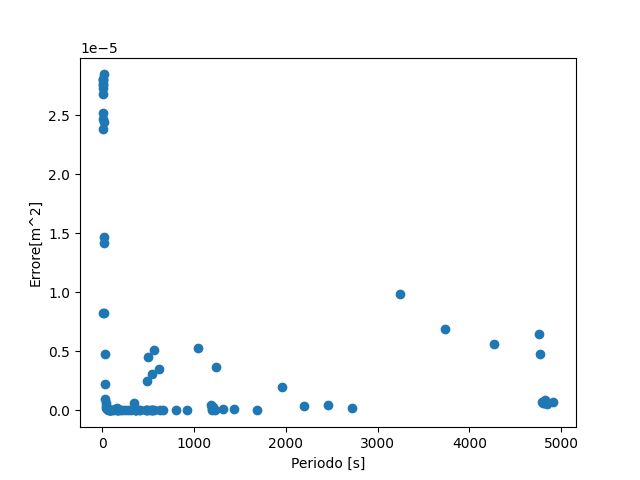
\includegraphics[scale=0.70]{img/puls0010/puntoUtopia10.png}
    \caption{Regione paretiana per problema da 10 punti di tabella \ref{tab:fuori_}}
    \label{fig:reg_ammis_10_0010}
  \end{figure}

  \begin{figure}[H]
    \centering
    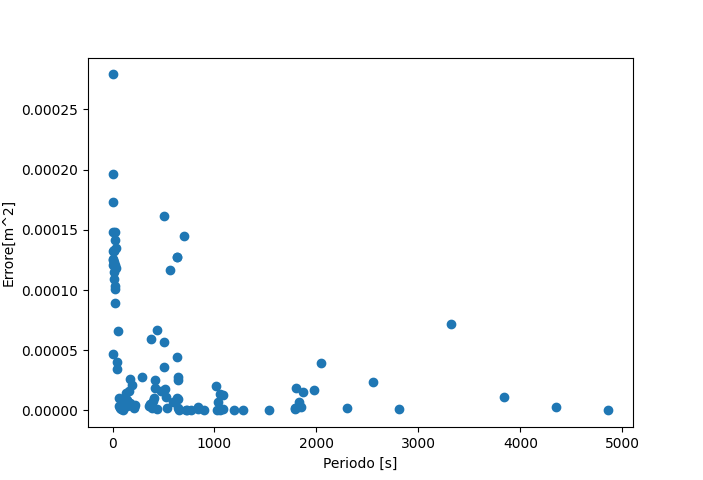
\includegraphics[scale=0.70]{img/puls0010/puntoUtopia20.png}
    \caption{Regione paretiana per problema da 20 punti di tabella \ref{tab:fuori_}}
    \label{fig:reg_ammis_20_0010}
  \end{figure}

  \begin{figure}[H]
    \centering
    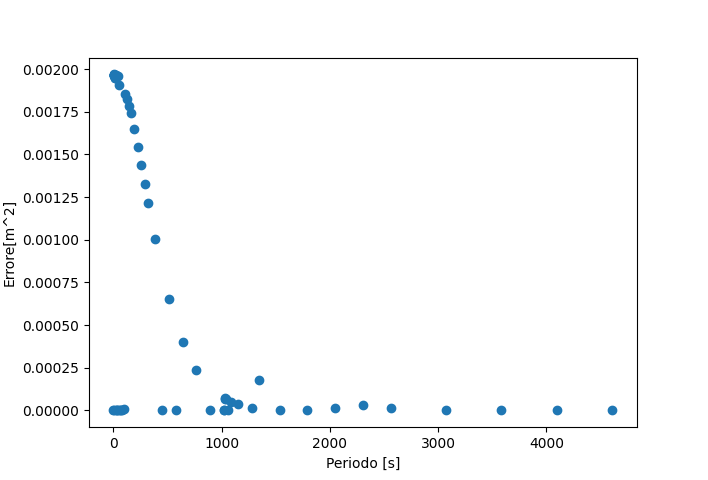
\includegraphics[scale=0.70]{img/puls0010/puntoUtopia30.png}
    \caption{Regione paretiana per problema da 30 punti di tabella \ref{tab:fuori_}}
    \label{fig:reg_ammis_30_0010}
  \end{figure}

  \item $ e(t)~=~sin(0.0013t)$ sinusoide con periodo pari a:
  $T = 4830.7s$
  \begin{table}[H]
    \caption{periodo da individuare uguale a 4830.7s}
    \label{tab:limiteSup_}
    \begin{center}
      \begin{tabularx}{\textwidth}{SSSp{0.5\textwidth}}
        \toprule
        {Numero di punti} & {Periodo della soluzione (s)} & {Tempo di calcolo (s)} & {Errore quadratico \newline medio ($m^2$)}\\
        \midrule
        10 &  1201 & 7.5 & $\expnumber{1.3}{-11}$\\
        20 &  2095 & 10.3 & $\expnumber{7.5}{-5}$\\
        30 &  4175 & 10.9 & $\expnumber{3.2}{-4}$\\
        \bottomrule
      \end{tabularx}
    \end{center}
  \end{table}

  \begin{figure}[H]
    \centering
    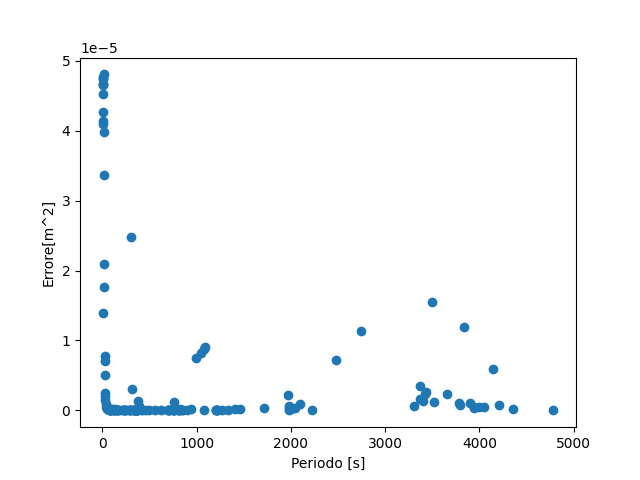
\includegraphics[scale=0.70]{img/puls0013/puntoUtopia10.png}
    \caption{Regione paretiana per problema da 10 punti di tabella \ref{tab:limiteSup_}}
    \label{fig:reg_ammis_10_0013}
  \end{figure}

  \begin{figure}[H]
    \centering
    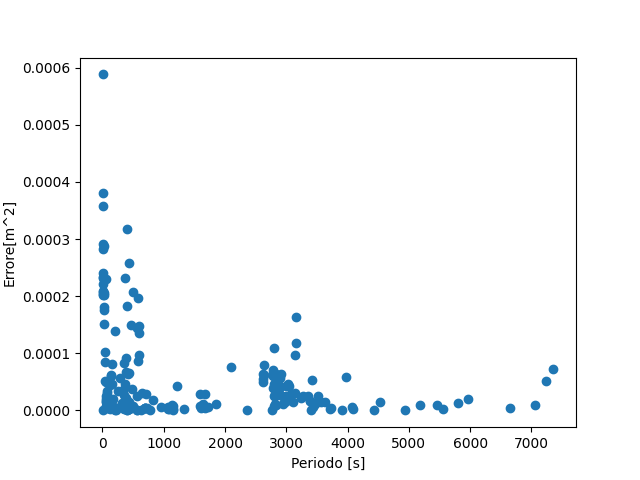
\includegraphics[scale=0.70]{img/puls0013/puntoUtopia20.png}
    \caption{Regione paretiana per problema da 20 punti di tabella \ref{tab:limiteSup_}}
    \label{fig:reg_ammis_20_0013}
  \end{figure}

  \begin{figure}[H]
    \centering
    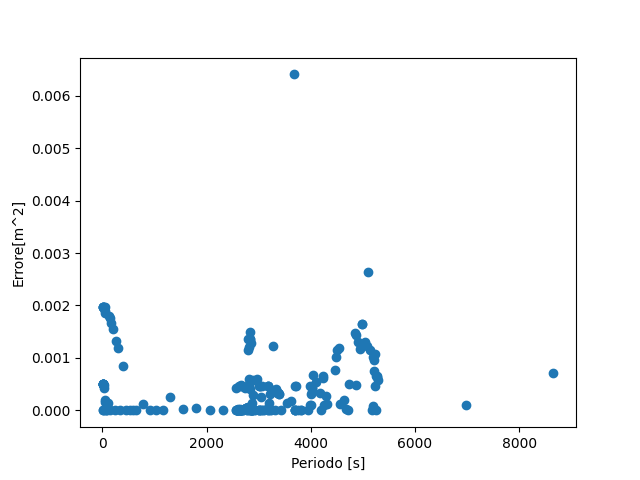
\includegraphics[scale=0.70]{img/puls0013/puntoUtopia30.png}
    \caption{Regione paretiana per problema da 30 punti di tabella \ref{tab:limiteSup_}}
    \label{fig:reg_ammis_30_0013}
  \end{figure}


  \item $ e(t)~=~sin(0.005t)$ sinusoide con periodo pari a:
    T = 1256s
  \begin{table}[H]
    \caption{periodo da individuare uguale a 1256s}
    \label{tab:centro1_}
    \begin{center}
      \begin{tabularx}{\textwidth}{SSSp{0.5\textwidth}}
        \toprule
        {Numero di punti} & {Periodo della soluzione (s)} & {Tempo di calcolo (s)} & {Errore quadratico \newline medio ($m^2$)}\\
        \midrule
        10 &  753  & 6.8 & $\expnumber{1.3}{-6}$\\
        20 &  1321 & 16.2 & $\expnumber{1.7}{-4}$\\
        30 &  1681 & 8.2 & $\expnumber{9.6}{-4}$\\
        \bottomrule
      \end{tabularx}
    \end{center}
  \end{table}

  \begin{figure}[H]
    \centering
    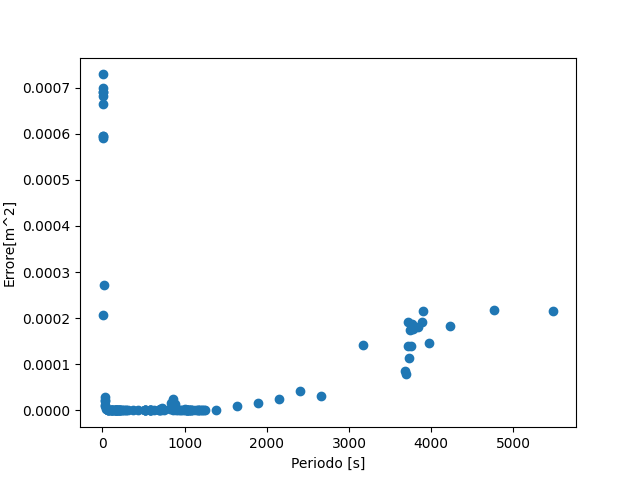
\includegraphics[scale=0.70]{img/puls005/puntoUtopia10.png}
    \caption{Regione paretiana per problema da 10 punti di tabella \ref{tab:centro1_}}
    \label{fig:reg_ammis_10_005}
  \end{figure}

  \begin{figure}[H]
    \centering
    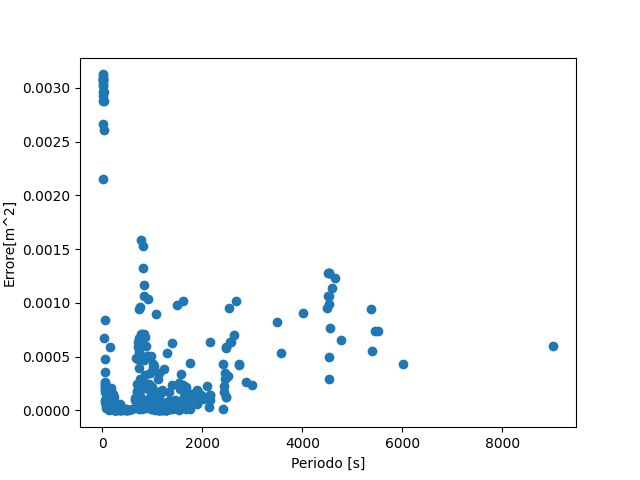
\includegraphics[scale=0.70]{img/puls005/puntoUtopia20.png}
    \caption{Regione paretiana per problema da 20 punti di tabella \ref{tab:centro1_}}
    \label{fig:reg_ammis_20_005}
  \end{figure}

  \begin{figure}[H]
    \centering
    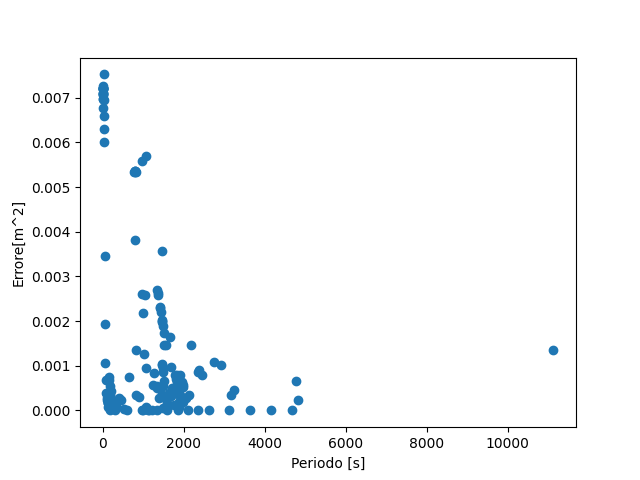
\includegraphics[scale=0.70]{img/puls005/puntoUtopia30.png}
    \caption{Regione paretiana per problema da 30 punti di tabella \ref{tab:centro1_}}
    \label{fig:reg_ammis_30_005}
  \end{figure}

  \item $ e(t)~=~sin(0.0125t)$ sinusoide con periodo pari a:
      T = 502.4s

    \begin{table}[H]
      \caption{periodo da individuare uguale a 502.4s}
      \label{tab:centro2_}
      \begin{center}
      \begin{tabularx}{\textwidth}{SSSp{0.5\textwidth}}
        \toprule
        {Numero di punti} & {Periodo della soluzione (s)} & {Tempo di calcolo (s)} & {Errore quadratico \newline medio ($m^2$)}\\
        \midrule
        10 &  425  & 6.4 & $\expnumber{2.5}{-10}$\\
        20 &  701 & 18.1 & $\expnumber{2.7}{-4}$\\
        30 &  589 & 9.3 & $\expnumber{6.0}{-4}$\\
        \bottomrule
      \end{tabularx}
      \end{center}
    \end{table}
    \begin{figure}[H]
      \centering
      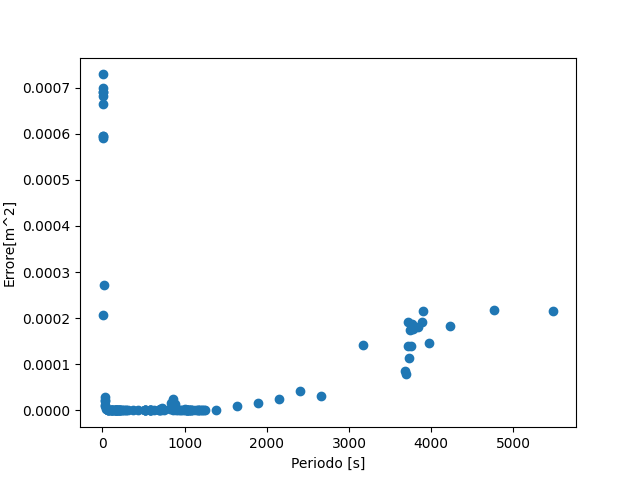
\includegraphics[scale=0.70]{img/puls005/puntoUtopia10.png}
      \caption{Regione paretiana per problema da 10 punti di tabella \ref{tab:centro2_}}
      \label{fig:reg_ammis_10_0125}
    \end{figure}

    \begin{figure}[H]
      \centering
      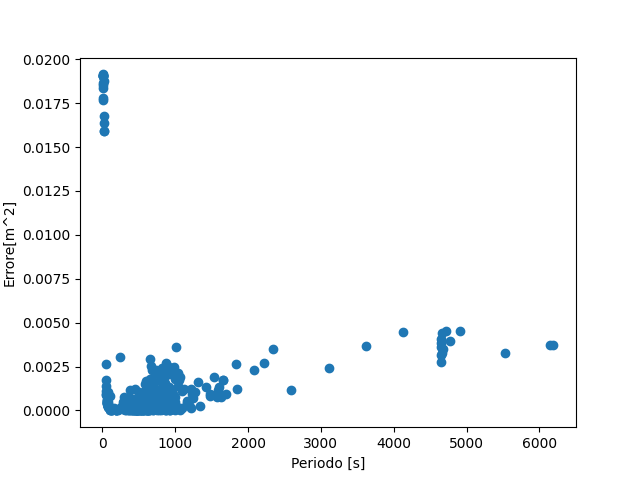
\includegraphics[scale=0.70]{img/puls0125/puntoUtopia20.png}
      \caption{Regione paretiana per problema da 20 punti di tabella \ref{tab:centro2_}}
      \label{fig:reg_ammis_20_0125}
    \end{figure}

    \begin{figure}[H]
      \centering
      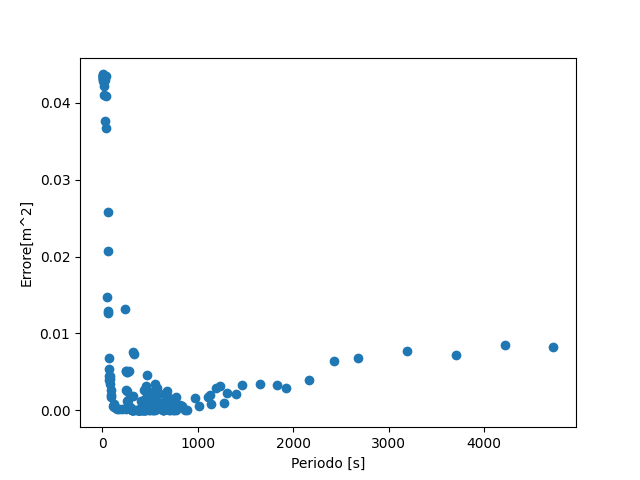
\includegraphics[scale=0.70]{img/puls0125/puntoUtopia30.png}
      \caption{Regione paretiana per problema da 30 punti di tabella \ref{tab:centro2_}}
      \label{fig:reg_ammis_30_0125}
    \end{figure}
    \item $ e(t)~=~sin(0.8t)$ sinusoide con periodo pari a:
        T = 7.85s
      \begin{table}[H]
        \caption{periodo da individuare uguale a 7.85s}
        \begin{center}
          \label{tab:limiteInf_}
          \begin{tabularx}{\textwidth}{SSSp{0.5\textwidth}}
            \toprule
            {Numero di punti} & {Periodo della soluzione (s)} & {Tempo di calcolo (s)} & {Errore quadratico \newline medio ($m^2$)}\\
            \midrule
            10 &  40  & 2.2 & $\expnumber{1.3}{-6}$\\
            20 &  8313 & 97.0 & $\expnumber{1.7}{-4}$\\
            30 &  4519 & 12.1 & $\expnumber{9.6}{-4}$\\
            \bottomrule
          \end{tabularx}
        \end{center}
      \end{table}
\end{itemize}

L'esecuzione dell'algoritmo è caratterizzato da uno scostamento medio dal periodo da individuare di $2377s$ e una mediana di $1278s$ ed infine un tempo medio di esecuzione di $13.62s$ e una mediana di $6.8s$.

La mediana e la media dello scostamento denotano un alta differenza tra la soluzione scelta dall'algoritmo e la sinusoide del problema, la causa di ciò è da individuarsi nel posizionamento del punto di utopia ed una mancata normalizzazione dei domini dell'errore e periodo.

Prendendo ad esempio la tabella \ref{tab:centro1_}, in particolare la soluzione individuata per il problema da 20 punti ed suo il grafico delle soluzioni generate, figura \ref{fig:tutte_le_soluzioni} e figura \ref{fig:soluzione_corretta}, si può notare che una soluzione con scostamento minore è stata individuata, ma non scelta dall'algoritmo di selezione poiché la distanza euclidea dal punto di utopia risulta maggiore rispetto alla soluzione scelta.

Legenda per i grafici da figura \ref{fig:tutte_le_soluzioni} a figura \ref{fig:da_zero_a_venti}:
\begin{itemize}
  \item 
\includegraphics{img/utility/matplotlib_markers/soluzione.png}: soluzione individuata.
  \item 
\includegraphics{img/utility/matplotlib_markers/soluzione_scelta.png}: soluzione individuata scelta dal criterio.
  \item 
\includegraphics{img/utility/matplotlib_markers/punto_utopia.png}:
  punto di utopia.
  \item 
\includegraphics{img/utility/matplotlib_markers/soluzione_ideale.png}: soluzione individuata ideale.
  \item 
\includegraphics{img/utility/matplotlib_markers/punto_sinusoide.png}: punto della sinusoide del problema.
\end{itemize}
\begin{figure}
  \center
  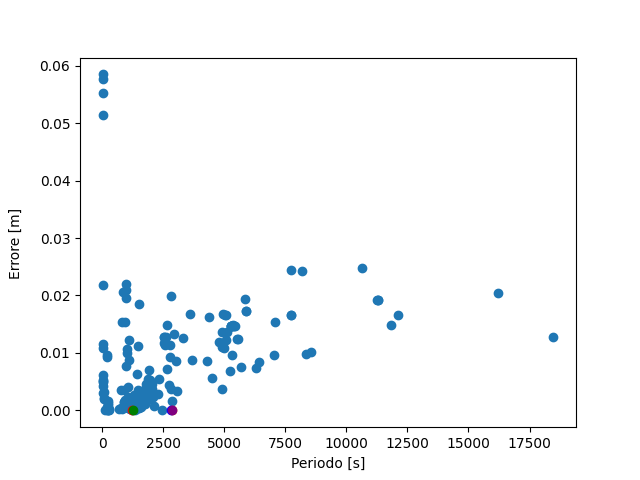
\includegraphics[scale=0.70]{img/puls005/tutte_le_soluzioni.png}
  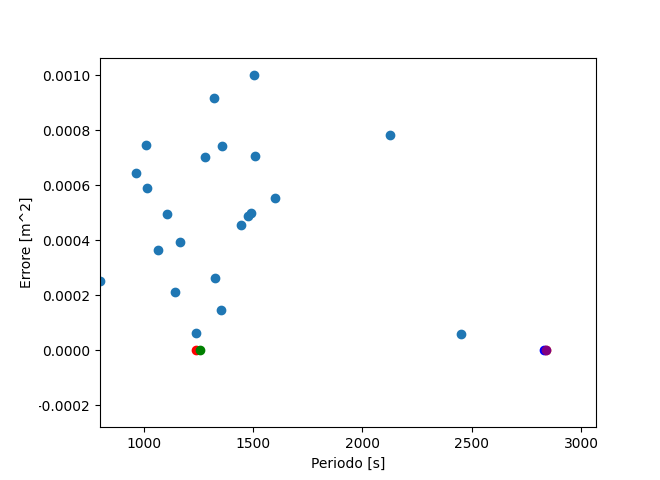
\includegraphics[scale=0.70]{img/puls005/tutte_le_soluzioni_2.png}
  \caption{Soluzioni generate per il problema di \ref{tab:centro1_} con 20 punti}
  \label{fig:tutte_le_soluzioni}
\end{figure}

\begin{figure}
  \center
  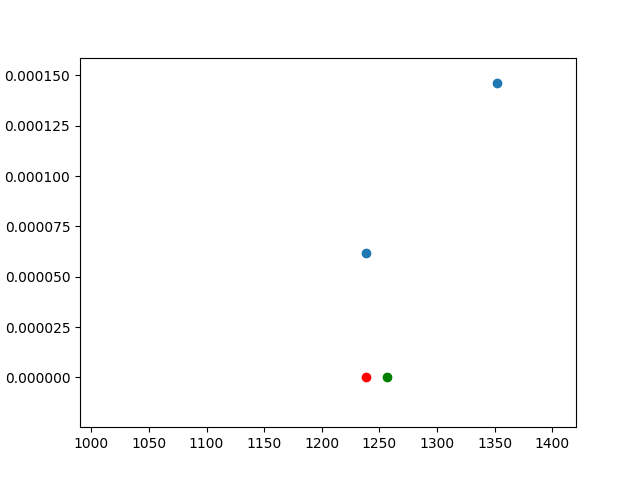
\includegraphics[scale=0.70]{img/puls005/soluzione_corretta.png}
  \caption{soluzione ideale per il problema di tabella \ref{tab:centro1_} con 20 punti}
  \label{fig:soluzione_corretta}
\end{figure}


\begin{figure}
  \center
  
\includegraphics[scale=0.70]{img/puls005/soluzione_scelta.png}
  \caption{soluzione scelta per il problema di tabella \ref{tab:centro1_} con 20 punti}
  \label{fig:soluzione_scelta}
\end{figure}
Da come si può notare dal primo grafico di figura \ref{fig:tutte_le_soluzioni} il punto di utopia risulta essere traslato al di fuori della zona dove la maggior parte delle soluzioni sono situate, a causa di soluzioni outlier.

È necessario quindi implementare un metodo di determinazione del periodo del punto di utopia migliore o passare ad un altro criterio di selezione.

Un miglioramento può essere l'implementazione di una media pesata, dove si determina il peso in base al errore della soluzione, questo permette di dare più rilevanza alle soluzioni con errore minore, comprendendo però in questo modo anche soluzioni con basso periodo rispetto al periodo della sinusoide da individuare.

Una soluzione alternativa può essere la modifica dell'algoritmo di controllo ed esplorazione dei periodi, modificando la gestione del passo. Diminuendo il passo quando si individua una soluzione con errore minore di un determinato valore di soglia, si approfondisce e si aumenta il numero di soluzioni individuate in un intorno di esso.

L'altra probabile causa è la mancata normalizzazione dei domini dell'errore e del periodo. Si possono notare gli effetti di ciò nel grafico in figura \ref{fig:tutte_le_soluzioni_08} corrispondente alla tabella \ref{tab:limiteInf_} per il problema da 20 punti.

\begin{figure}
  \center
  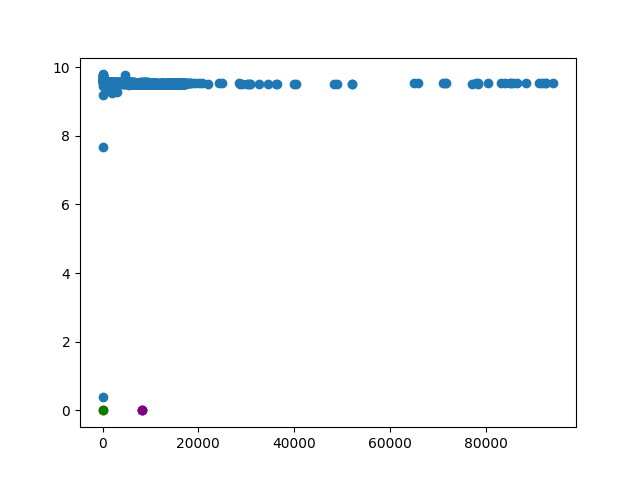
\includegraphics[scale=0.80]{img/puls08/tutte_le_soluzioni.png}
  \caption{Soluzioni generate per il problema di tabella \ref{tab:limiteInf_} con 20 punti}
  \label{fig:tutte_le_soluzioni_08}
\end{figure}

Si può notare, dai grafici in figura \ref{fig:soluzione_ideale_08} e \ref{fig:posizione_utopia_08} che la distanza tra il punto di utopia e la soluzione con periodo che si scosta meno dalla soluzione da individuare, è approssimatamente pari ad un valore di 8000s, molto maggiore rispetto ad una soluzione che ha lo stesso periodo del punto di utopia ma con uno scostamento maggiore, pari a 9.5

\begin{figure}
  \center
  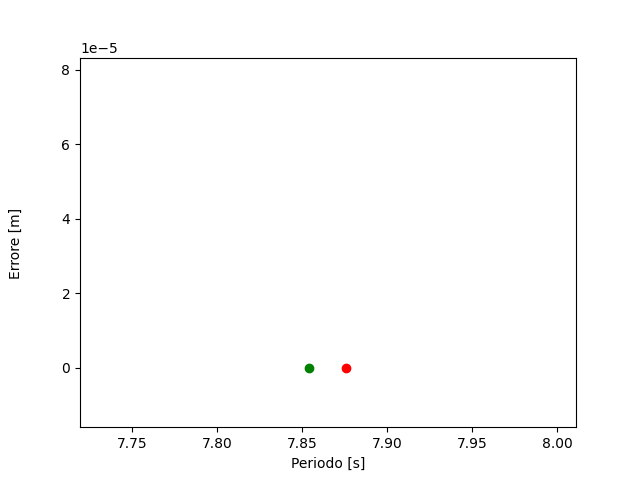
\includegraphics[scale=0.70]{img/puls08/soluzione_corretta.png}
  \caption{Soluzione ideale per il problema di \ref{tab:limiteInf_} con 20 punti}
  \label{fig:soluzione_ideale_08}
\end{figure}

\begin{figure}
  \center
  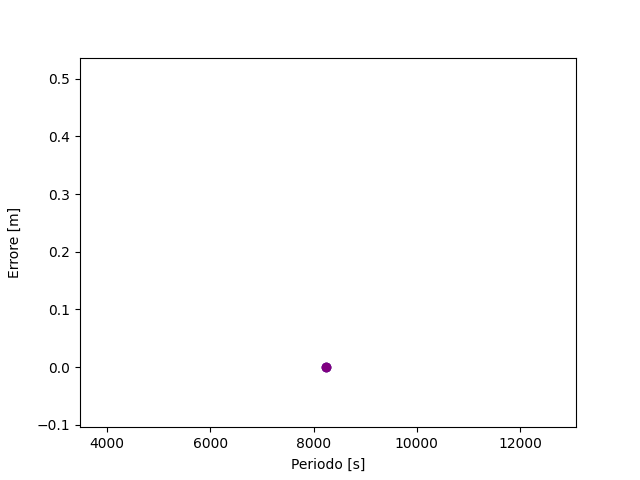
\includegraphics[scale=0.70]{img/puls08/posizione_utopia.png}
  \caption{Posizione del punto di utopia per il problema di \ref{tab:limiteInf_} con 20 punti}
  \label{fig:posizione_utopia_08}
\end{figure}




Un altro fattore che ha determinato la mancata scelta della soluzione ideale, mostrata in figura \ref{fig:soluzione_ideale_08}, sono il numero di soluzioni individuate in un suo intorno limitato, come per esempio nell'insieme dei periodi [0, 20] illustrato in figura \ref{fig:da_zero_a_venti}, dove sono individuate solo 6 soluzioni rispetto al numero totale di soluzioni individuate pari a 1527 in questo esempio.

Il problema di questa metodologia di specifica del periodo per il punto di utopia è che è basata in maniera marcata sulle prestazioni, il numero e la tipologia di soluzioni individuate dall'algoritmo di esplorazione dei periodi.

\begin{figure}
  \center
  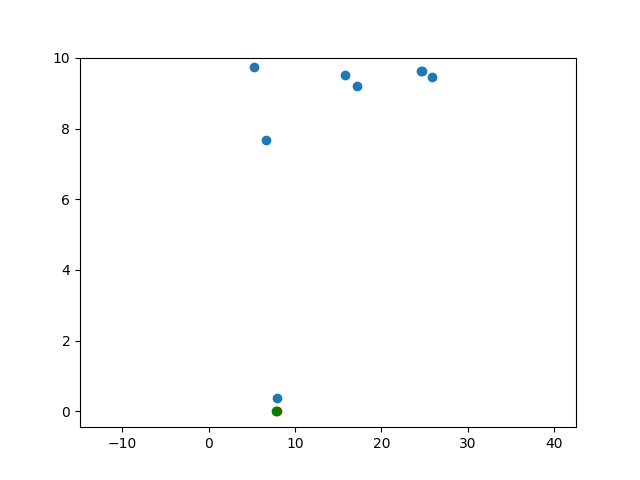
\includegraphics[scale=0.70]{img/puls08/da_zero_a_venti.png}
  \caption{Soluzioni individuate nell'insieme di periodi [0, 20] per il problema di tabella \ref{tab:limiteInf_} con 20 punti}
  \label{fig:da_zero_a_venti}
\end{figure}

Riassumendo, per il miglioramento del criterio di selezione esplicito le seguenti possibili modifiche:
\begin{itemize}
  \item La normalizzazione dei domini di errore e di periodo per tutte le soluzioni individuate
  \item L'implementazione di una media pesata e quindi il calcolo del peso per ogni soluzione individuata in base al suo errore.
  \item Aggiunta di condizione di diminuzione del passo nel algoritmo esplorazione dei periodi.
\end{itemize}

Dato le ampie modifiche richieste, ho optato per l'individuazione e definizione di un altro criterio di selezione.

\subsubsection{Criterio degli standard sull'errore}
\label{sss:standard}
Gli standard sono valori-soglia al di sotto dei quali non si vuole che gli
obiettivi possano peggiorare. Data la non predicibilità del periodo ottimale in questo problema, è possibile definire gli standard solo per l'errore. La modalità con il quale ho definito gli standard per la scelta della soluzione prevede la suddivisione in range del dominio dell'errore, ipotizzando che ogni soluzione in uno stesso range sia equivalente, se si considera solo l'errore. Ogni range è identificato con un numero ordinale specificandoli come livelli: primo livello, secondo livello, ... , n-esimo livello, dove per ordine crescente dei livelli si ha l'aumento del range d'errore. I range devono essere definiti a priori, in maniera attenta rispetto all'errore intriseco dello strumento di rilevazione dei punti. È necessario inoltre effettuare ipotesi sul errore di una soluzione: errore di una soluzione ottimale, errore di una soluzione non correlata ai punti, errore di una soluzione legata ad un sottoproblema con un assegnamento di punti errato.

Il seguente pseudocodice illustra una procedura di una struttura dati che ho definito, per contenere la soluzione con livello più basso possibile e con più alto periodo tra tutte le soluzioni individuate all'interno del corrispettivo livello, perciò gli standard dell'errore sono fissati dalla soluzione con il livello minore.
\begin{algorithm}
\SetKwInOut{Input}{input}\SetKwInOut{Output}{output}
\SetKwComment{Comment}{/* }{ */}
\SetKwData{SolOttimale}{solOttimale}
\SetKwData{SolCorrente}{solCorrente}
\SetKwData{UltimoLv}{ultimoLv}
\SetKwFunction{LivelloDi}{LivelloDi}
\caption{Criterio degli standard}\label{alg: standard}
\Input{\SolCorrente tupla contenente ($errore,~periodo,~ampiezza,~fase$)}
\eIf{\LivelloDi{\SolCorrente} $<$ \LivelloDi{\SolOttimale}}{ \label{std:min}
    $\SolOttimale \gets \SolCorrente$\\
}{\If{\LivelloDi{\SolCorrente} $=$ \LivelloDi{\SolOttimale}}{
      \eIf{\LivelloDi{\SolCorrente} $=$ \UltimoLv } {
          \If{$\SolCorrente[errore] < \SolOttimale[errore]$}{ \label{std:last}
              $\SolOttimale \gets \SolCorrente$\\
          }
       } {
          \If{$\SolCorrente[periodo] > \SolOttimale[periodo]$}{ \label{std:per}
              $\SolOttimale \gets \SolCorrente$\\
          }
       }
  }
}
\end{algorithm}

Tutte le soluzioni con un livello maggiore della soluzione ottimale vengono scartate (riga \ref{std:min}, algoritmo \ref{alg: standard}), invece se la soluzione corrente ha un livello inferiore, essa viene memorizzata come soluzione ottimale. Se i livelli della soluzione ottimale e della soluzione corrente si equivalgono, si memorizza la soluzione corrente solo se essa ha un periodo maggiore della soluzione ottimale (riga \ref{std:per}, algoritmo \ref{alg: standard}).

Solo l'ultimo livello ha un criterio di selezione della soluzione ottimale differente, poiché si seleziona la soluzione con il minimo errore (riga \ref{std:last}, algoritmo \ref{alg: standard}). L'ultimo livello,  rappresenta l'insieme dei valori d'errore più alti, che vanno da un valore fissato a $+\infty$, perciò all'interno di questo insieme illimitato, cerco di selezionare la soluzione che più si correla all'assegnamento dei punti.

Illustro i risultati dell'implementazione ed esecuzione del criterio degli standard, generando le soluzioni utilizzando il modello basato sul metodo dei vincoli, variando il minimo periodo $\beta$ nel range fissato (sezione \ref{ss:arresto}).

I livelli fissati sono
\begin{itemize}
  \item Livello 1: errore $<$ $\expnumber{1}{-5}$
  \item Livello 2: errore $<$ $\expnumber{1}{-2}$
  \item Livello 3: errore $<$ $\expnumber{1}{-1}$
  \item Livello 4: errore $<$ 1
  \item Livello 5: errore $<$ 3
  \item Livello 6: errore $<$ 5
  \item Livello 7: errore $<$ 7
  \item Livello 8: errore $<$ 10
  \item Livello 9: errore $\geq$ 10
\end{itemize}
Ho fissato i range in maniera da ottenere maggiore precisione e diversificazione delle soluzioni con errore tra 0 e 1, suddividento tale spazio in 4 livelli. Nella definizione dei livelli, non ho tenuto in cosiderazione l'errore intrinseco dello strumento di rilevazione, per ottenere delle prime informazioni sulla prestazione dell'algoritmo in una situazione ideale. A seguito si elencano problemi con punti generati da una sinusoide e(t) e nelle tabelle le soluzioni individuate dall'algoritmo.

I parametri dell'algoritmo \ref{controlloErrore} per le seguenti sperimentazioni sono:
\begin{itemize}
  \item $f(x)$ in riga \ref{velocitaPasso}, algoritmo \ref{controllo} pari alla funzione \eqref{velocitaPassoEspl} con $k = 5$
  \item $periodoIniziale = 0s$
  \item $periodoFinale = 5000s$
  \item $tolleranzaDefault = \expnumber{1}{-6}$
\end{itemize}

\begin{itemize}
  \item $ e(t)~=~sin(0.0010t)$ sinusoide con periodo pari~a: $T = \frac{2\pi}{\omega} = \frac{2\pi}{0.0010} = 6280s$
  \begin{table}[H]
    \caption{periodo da individuare uguale a 6280s}
    \label{tab:fuori}
    \begin{center}
      \begin{tabularx}{\textwidth}{SSSp{0.5\textwidth}}
        \toprule
        {Numero di punti} & {Periodo della soluzione (s)} & {Tempo di calcolo (s)} & {Errore quadratico \newline medio ($m^2$)}\\
        \midrule
        % 1648.2 % 694.6 % 1374
        10 &  4631.8  & 2.2 & $\expnumber{9.0}{-7}$\\
        20 &  5585.4 & 1.9 & $\expnumber{1.0}{-34}$\\
        30 &  4906.0 & 2.0 & $\expnumber{6.0}{-4}$\\
        \bottomrule
      \end{tabularx}
    \end{center}
  \end{table}

  \begin{figure}[H]
    \centering
    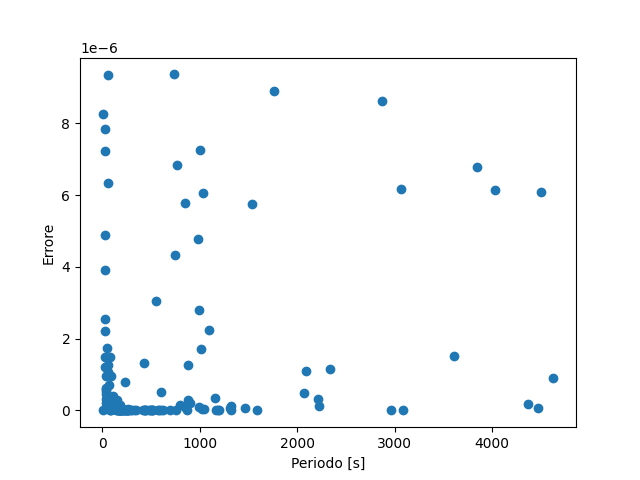
\includegraphics[scale=0.70]{img/puls0010/standard10.png}
    \caption{Regione paretiana per problema da 10 punti di tabella \ref{tab:fuori}}
    \label{fig:reg_ammis_10_0010_std}
  \end{figure}

  \begin{figure}[H]
    \centering
    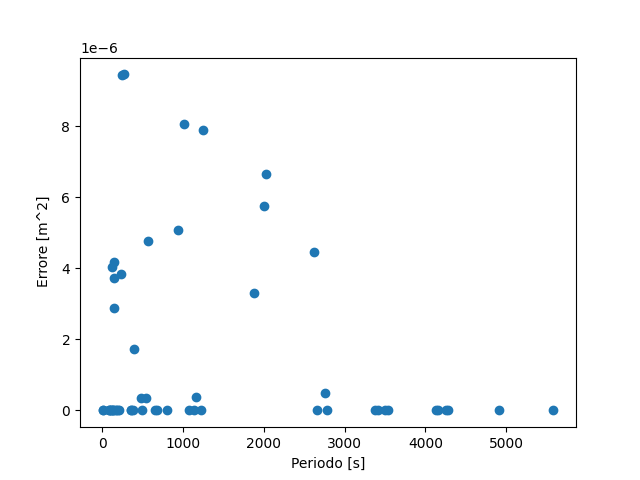
\includegraphics[scale=0.70]{img/puls0010/standard20.png}
    \caption{Regione paretiana per problema da 20 punti di tabella \ref{tab:fuori}}
    \label{fig:reg_ammis_20_0010_std}
  \end{figure}

  \begin{figure}[H]
    \centering
    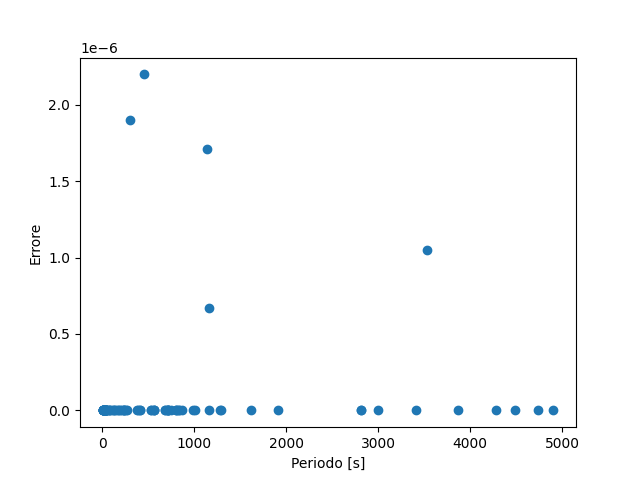
\includegraphics[scale=0.70]{img/puls0010/standard30.png}
    \caption{Regione paretiana per problema da 30 punti di tabella \ref{tab:fuori}}
    \label{fig:reg_ammis_30_0010_std}
  \end{figure}


  \item $ e(t)~=~sin(0.0013t)$ sinusoide con periodo pari a:
  $T = 4830.7s$
  \begin{table}[H]
    \caption{periodo da individuare uguale a 4830.7s}
    \label{tab:limiteSup}
    \begin{center}
      \begin{tabularx}{\textwidth}{SSSp{0.5\textwidth}}
        \toprule
        {Numero di punti} & {Periodo della soluzione (s)} & {Tempo di calcolo (s)} & {Errore quadratico \newline medio ($m^2$)}\\
        \midrule
        % 359.7 % 76.3 % 338.7
        10 &  4471.5  & 2.2 & $\expnumber{6.4}{-8}$\\
        20 &  4907.0 & 2.0 & $0.0$\\
        30 &  4492.0 & 2.3 & $0.0$\\
        \bottomrule
      \end{tabularx}
    \end{center}
  \end{table}

  \begin{figure}[H]
    \centering
    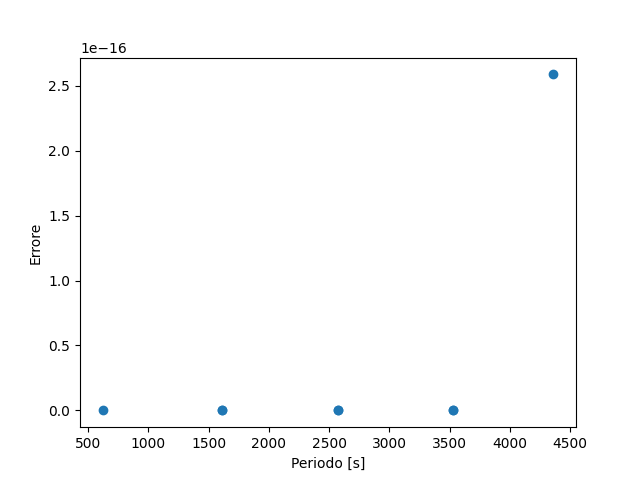
\includegraphics[scale=0.70]{img/puls0013/standard10.png}
    \caption{Regione paretiana per problema da 10 punti di tabella \ref{tab:limiteSup}}
    \label{fig:reg_ammis_10_0013_std}
  \end{figure}

  \begin{figure}[H]
    \centering
    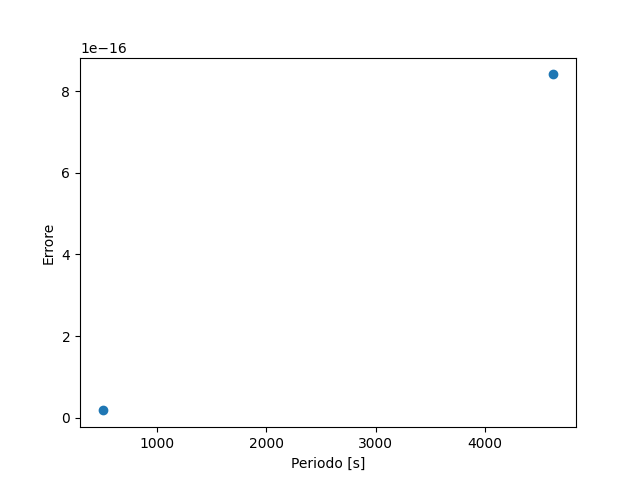
\includegraphics[scale=0.70]{img/puls0013/standard20.png}
    \caption{Regione paretiana per problema da 20 punti di tabella \ref{tab:limiteSup}}
    \label{fig:reg_ammis_20_0013_std}
  \end{figure}

  \begin{figure}[H]
    \centering
    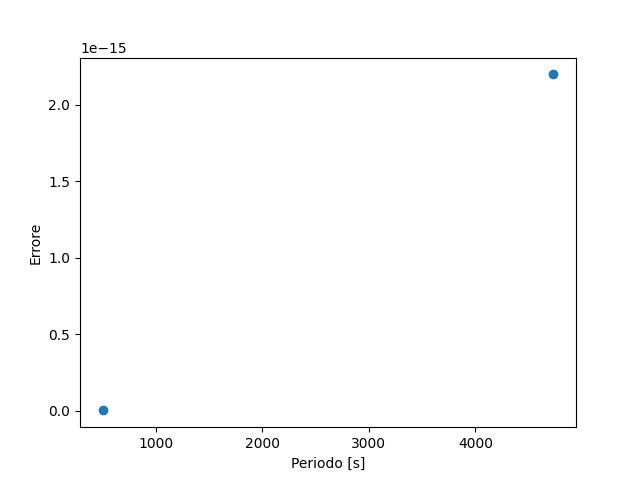
\includegraphics[scale=0.70]{img/puls0013/standard30.png}
    \caption{Regione paretiana per problema da 30 punti di tabella \ref{tab:limiteSup}}
    \label{fig:reg_ammis_30_0013_std}
  \end{figure}


  \item $ e(t)~=~sin(0.005t)$ sinusoide con periodo pari a:
    T = 1256s
  \begin{table}[H]
    \caption{periodo da individuare uguale a 1256s}
    \label{tab:centro1}
    \begin{center}
      \begin{tabularx}{\textwidth}{SSSp{0.5\textwidth}}
        \toprule
        {Numero di punti} & {Periodo della soluzione (s)} & {Tempo di calcolo (s)} & {Errore quadratico \newline medio ($m^2$)}\\
        \midrule
        % 503 % 32 % 3484
        10 &  1759.0  & 2.1 & $\expnumber{8.9}{-6}$\\
        20 &  1224.0 & 2.6 & $0.0$\\
        30 &  4740 & 2.0 & $0.0$\\
        \bottomrule
      \end{tabularx}
    \end{center}
  \end{table}

  \begin{figure}[H]
    \centering
    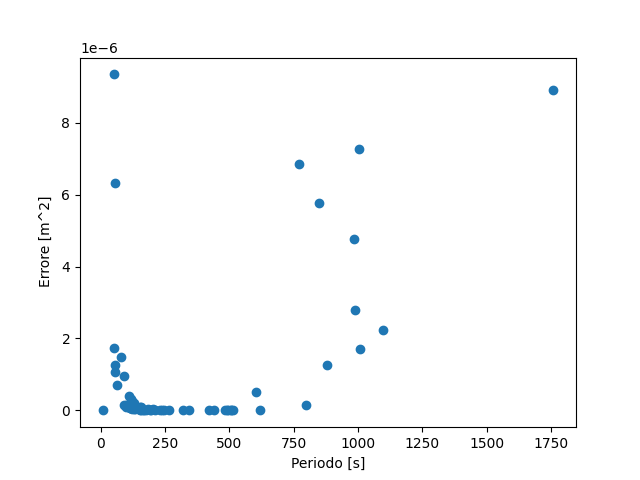
\includegraphics[scale=0.70]{img/puls005/standard10.png}
    \caption{Regione paretiana per problema da 10 punti di tabella \ref{tab:centro1}}
    \label{fig:reg_ammis_10_005_std}
  \end{figure}

  \begin{figure}[H]
    \centering
    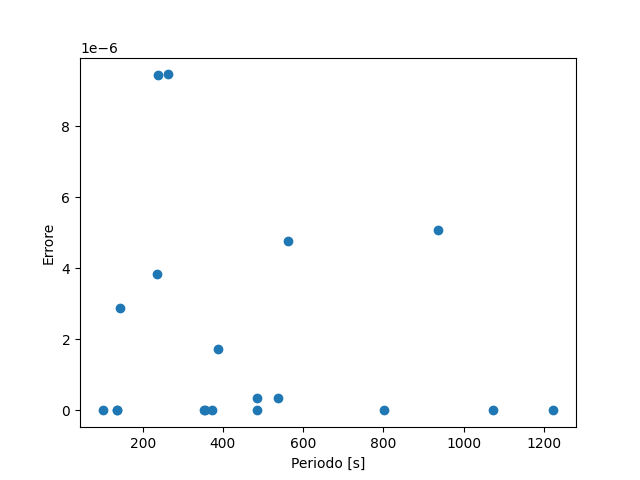
\includegraphics[scale=0.70]{img/puls005/standard20.png}
    \caption{Regione paretiana per problema da 20 punti di tabella \ref{tab:centro1}}
    \label{fig:reg_ammis_20_005_std}
  \end{figure}

  \begin{figure}[H]
    \centering
    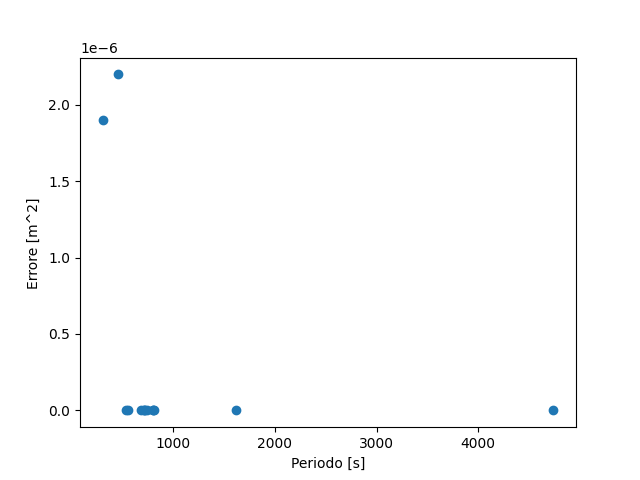
\includegraphics[scale=0.70]{img/puls005/standard30.png}
    \caption{Regione paretiana per problema da 10 punti di tabella \ref{tab:centro1}}
    \label{fig:reg_ammis_30_005_std}
  \end{figure}

  \item $ e(t)~=~sin(0.0125t)$ sinusoide con periodo pari a:
      T = 502.4s

    \begin{table}[H]
      \caption{periodo da individuare uguale a 502.4s}
      \label{tab:centro2}
      \begin{center}
        \begin{tabularx}{\textwidth}{SSSp{0.5\textwidth}}
          \toprule
          {Numero di punti} & {Periodo della soluzione (s)} & {Tempo di calcolo (s)} & {Errore quadratico \newline medio ($m^2$)}\\
          \midrule
          % 99.6 % 299.3 % 240.6
          10 &  602.0  & 2.7 & $\expnumber{5.1}{-7}$\\
          20 &  801.9 & 6.0 & $0.0$\\
          30 &  743.0  & 2.2 & $0.0$\\
          \bottomrule
        \end{tabularx}
      \end{center}
    \end{table}

    \begin{figure}[H]
      \centering
      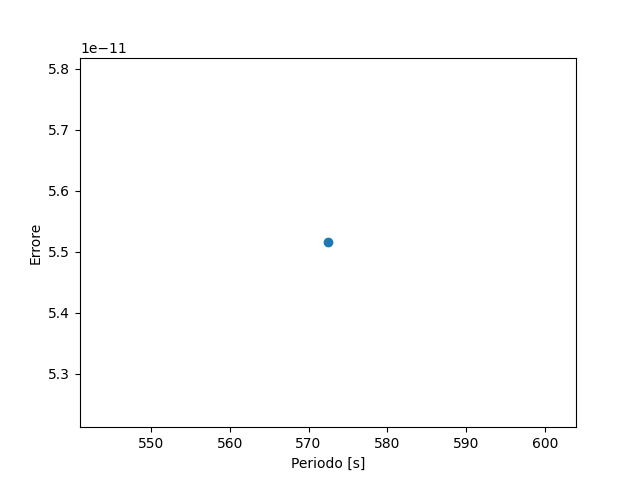
\includegraphics[scale=0.70]{img/puls0125/standard10.png}
      \caption{Regione paretiana per problema da 10 punti di tabella \ref{tab:centro2}}
      \label{fig:reg_ammis_10_0125_std}
    \end{figure}

    \begin{figure}[H]
      \centering
      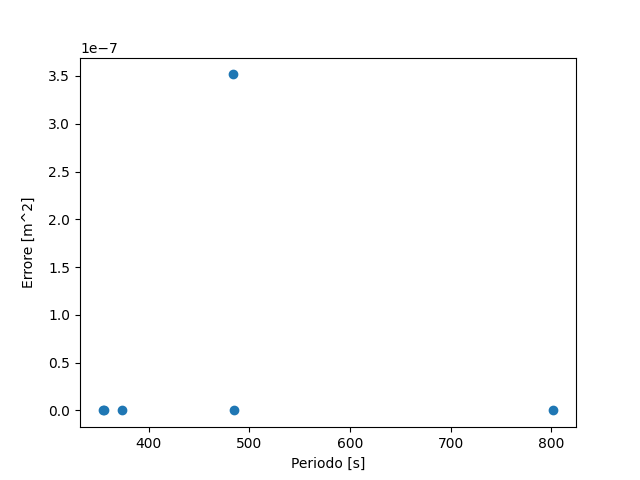
\includegraphics[scale=0.70]{img/puls0125/standard20.png}
      \caption{Regione paretiana per problema da 20 punti di tabella \ref{tab:centro2}}
      \label{fig:reg_ammis_20_0125_std}
    \end{figure}

    \begin{figure}[H]
      \centering
      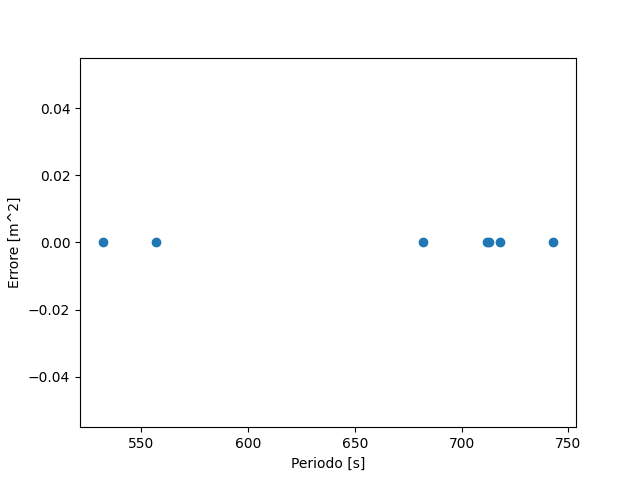
\includegraphics[scale=0.70]{img/puls0125/standard30.png}
      \caption{Regione paretiana per problema da 30 punti di tabella \ref{tab:centro2}}
      \label{fig:reg_ammis_30_0125_std}
    \end{figure}

    \item $ e(t)~=~sin(0.8t)$ sinusoide con periodo pari a:
        T = 7.85s



      \begin{table}[H]
        \caption{periodo da individuare uguale a 7.85s}
        \begin{center}
          \label{tab:limiteInf}
          \begin{tabularx}{\textwidth}{SSSp{0.5\textwidth}}
            \toprule
            {Numero di punti} & {Periodo della soluzione (s)} & {Tempo di calcolo (s)} & {Errore quadratico \newline medio ($m^2$)}\\
            \midrule
            % 0.05 % 0.15 %0.15
            10 &  7.8  & 1.8 & $\expnumber{5.0}{-9}$\\
            20 &  8.0 & 4.1 & $\expnumber{1.1}{-2}$\\
            30 &  8.0  & 2.5 & $\expnumber{2.5}{-2}$\\
            \bottomrule
          \end{tabularx}
        \end{center}
      \end{table}

      \begin{figure}[H]
        \centering
        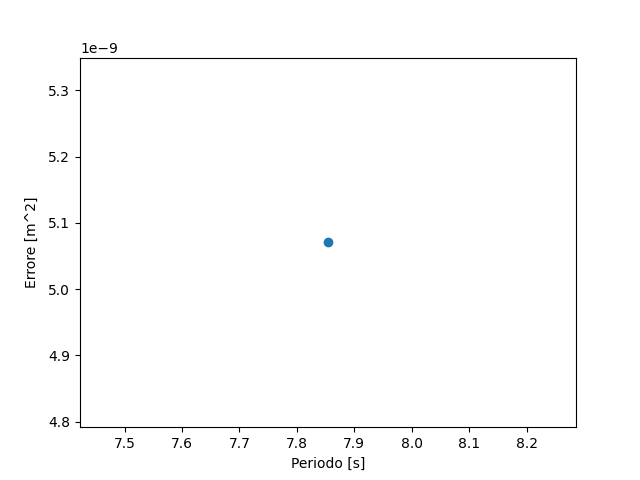
\includegraphics[scale=0.70]{img/puls08/standard10.png}
        \caption{Regione paretiana per problema da 10 punti di tabella \ref{tab:limiteInf}}
        \label{fig:reg_ammis_10_08_std}
      \end{figure}

      \begin{figure}[H]
        \centering
        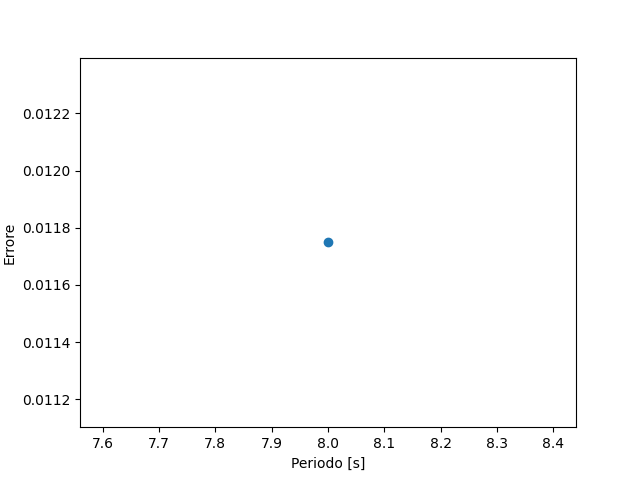
\includegraphics[scale=0.70]{img/puls08/standard20.png}
        \caption{Regione paretiana per problema da 10 punti di tabella \ref{tab:limiteInf}}
        \label{fig:reg_ammis_20_08_std}
      \end{figure}

      \begin{figure}[H]
        \centering
        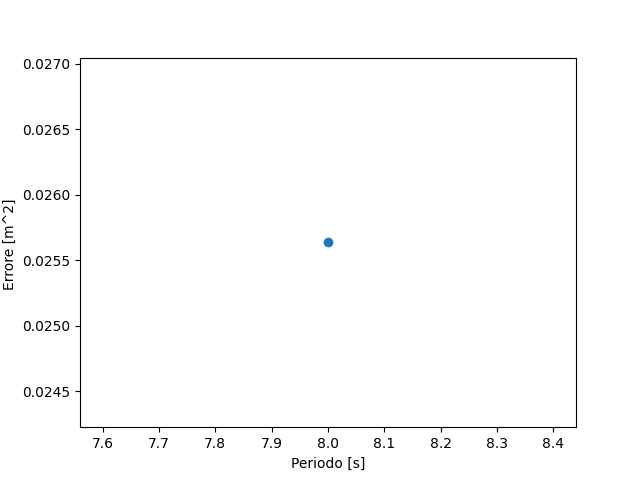
\includegraphics[scale=0.70]{img/puls08/standard30.png}
        \caption{Regione paretiana per problema da 30 punti di tabella \ref{tab:limiteInf}}
        \label{fig:reg_ammis_30_08_std}
      \end{figure}

\end{itemize}

L'esecuzione dell'algoritmo è caratterizzato da uno scostamento medio dal periodo da individuare di $610.0s$ e una mediana di $299.3s$ ed infine un tempo medio di esecuzione di $2.5s$ e una mediana di $2.2s$.

È possibile provare a diminuire il tempo di esecuzione modificando l'algoritmo di controllo ed esploranzione, aggiungendo come condizione di aumento del passo, l'individuazione di una soluzione dal livello maggiore di un livello di soglia. Questo permette una velocizzazione dell'esplorazione saltando tutti quei periodi di partenza lontani dal periodo della sinusoide da individuare.

Inoltre si può notare che l'errore delle soluzioni individuate si distribuisce in un range pari a $[0.0, \expnumber{2.5}{-2}]$, questo potrebbe suggerire  la definizione di livelli dai range più stringenti come ad esempio:

\begin{itemize}
  \item Livello 1: errore $<$ $\expnumber{1}{-9}$
  \item Livello 2: errore $<$ $\expnumber{1}{-7}$
  \item Livello 3: errore $<$ $\expnumber{1}{-5}$
  \item Livello 4: errore $<$ $\expnumber{1}{-3}$
  \item Livello 5: errore $<$ $\expnumber{1}{-1}$
  \item Livello 6: errore $<$ 1
  \item Livello 7: errore $<$ 3
  \item Livello 8: errore $<$ 5
  \item Livello 9: errore $\geq$ 5
\end{itemize}

Ma eseguendo i problemi da periodo elevato come i problemi di tabella \ref{tab:fuori} e \ref{tab:limiteSup}, si può notare nelle tabelle successive \ref{tab:fuori_stringente} e \ref{tab:limiteSup_stringente}, che le sinusoidi individuate per i problemi da 10 punti, si scostano mediamente di $4409.1s$ dalla sinusoide da individuare, evidenziando il problema delle sinusoidi da basso periodo rispetto alla sinusoide da individuare.

\begin{itemize}
  \item $ e(t)~=~sin(0.0010t)$ sinusoide con periodo pari~a: $T = \frac{2\pi}{\omega} = \frac{2\pi}{0.0010} = 6280s$
  \begin{table}[H]
    \caption{periodo da individuare uguale a 6280s}
    \label{tab:fuori_stringente}
    \begin{center}
      \begin{tabularx}{\textwidth}{SSSp{0.5\textwidth}}
        \toprule
        {Numero di punti} & {Periodo della soluzione (s)} & {Tempo di calcolo (s)} & {Errore quadratico \newline medio ($m^2$)}\\
        \midrule
        % 1648.2 % 694.6 % 1374
        10 &  1587.0  & 1.29 & $\expnumber{5.0}{-10}$\\
        20 &  4388 & 0.65 & $0.0$\\
        30 &  4907.0 & 0.9 & $0.0$ \\
        \bottomrule
      \end{tabularx}
    \end{center}
  \end{table}



  \item $ e(t)~=~sin(0.0013t)$ sinusoide con periodo pari a:
  $T = 4830.7s$
  \begin{table}[H]
    \caption{periodo da individuare uguale a 4830.7s}
    \label{tab:limiteSup_stringente}
    \begin{center}
      \begin{tabularx}{\textwidth}{SSSp{0.5\textwidth}}
        \toprule
        {Numero di punti} & {Periodo della soluzione (s)} & {Tempo di calcolo (s)} & {Errore quadratico \newline medio ($m^2$)}\\
        \midrule
        % 359.7 % 76.3 % 338.7
        10 &  704  & 2.2 & $\expnumber{6.4}{-8}$\\
        20 &  4478.0 & 0.77 & $0.0$\\
        30 &  4935.0 & 0.8 & $0.0$\\
        \bottomrule
      \end{tabularx}
    \end{center}
  \end{table}

  \begin{figure}[H]
    \centering
    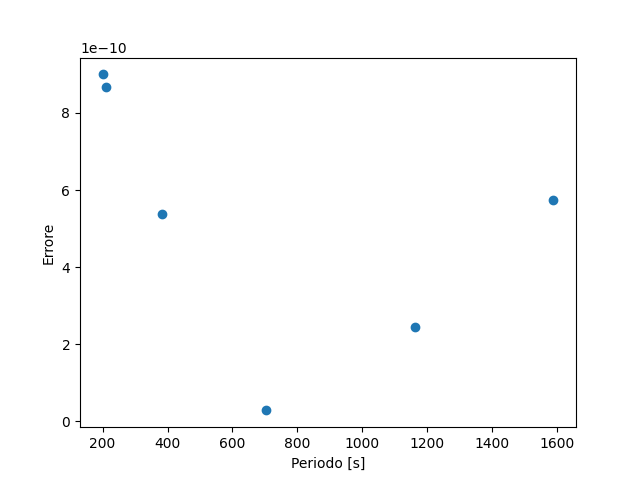
\includegraphics[scale=0.70]{img/puls0010/lv_stringenti10.png}
    \caption{Regione paretiana per problema da 10 punti di tabella \ref{tab:fuori_stringente}}
    \label{fig:reg_ammis_10_0010_stringente}
  \end{figure}

  \begin{figure}[H]
    \centering
    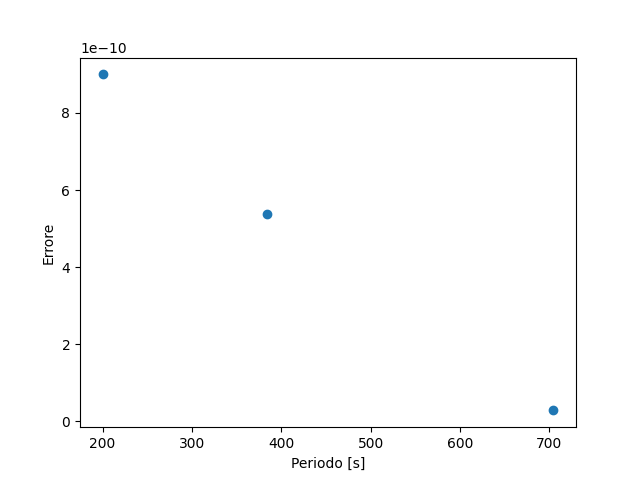
\includegraphics[scale=0.70]{img/puls0013/lv_stingenti10.png}
    \caption{Regione paretiana per problema da 10 punti di tabella \ref{tab:limiteSup_stringente}}
    \label{fig:reg_ammis_10_0013_stringente}
  \end{figure}
\end{itemize}

Perciò ho deciso di mantenere i livelli precedentemente definiti.

Infine un ulteriore modifica per l'accelerazione del l'algoritmo è agire sul parametro k della $f(x)$ in riga \ref{velocitaPasso}, algoritmo \ref{controllo}, fissandolo pari a $10$ il doppio del valore fissato precedentemente.

Effettuando questa modifiche e scegliendo come livello di soglia il quinto, si ottengono i seguenti risultati:
\begin{itemize}
  \item $ e(t)~=~sin(0.0010t)$ sinusoide con periodo pari~a: $T = \frac{2\pi}{\omega} = \frac{2\pi}{0.0010} = 6280s$
  \begin{table}[H]
    \caption{periodo da individuare uguale a 6280s}
    \label{tab:fuori_2}
    \begin{center}
      \begin{tabularx}{\textwidth}{SSSp{0.5\textwidth}}
        \toprule
        {Numero di punti} & {Periodo della soluzione (s)} & {Tempo di calcolo (s)} & {Errore quadratico \newline medio ($m^2$)}\\
        \midrule
        % 1669.2 % 1819 % 1374
        10 &  4610.8  & 1.2 & $\expnumber{9.8}{-7}$\\
        20 &  4461.0 & 1.2 & $0.0$\\
        30 &  4906.0 & 1.2 & $0.0$ \\
        \bottomrule
      \end{tabularx}
    \end{center}
  \end{table}


  \item $ e(t)~=~sin(0.0013t)$ sinusoide con periodo pari a:
  $T = 4830.7s$
  \begin{table}[H]
    \caption{periodo da individuare uguale a 4830.7s}
    \label{tab:limiteSup_2}
    \begin{center}
      \begin{tabularx}{\textwidth}{SSSp{0.5\textwidth}}
        \toprule
        {Numero di punti} & {Periodo della soluzione (s)} & {Tempo di calcolo (s)} & {Errore quadratico \newline medio ($m^2$)}\\
        \midrule
        % 248.7 % 111.3 % 369.7
        10 &  4582.0  & 1.0 & $\expnumber{4.3}{-8}$\\
        20 &  4942.0 & 1.2 & $0.0$\\
        30 &  4461.0 & 1.2 & $0.0$\\
        \bottomrule
      \end{tabularx}
    \end{center}
  \end{table}


  \item $ e(t)~=~sin(0.005t)$ sinusoide con periodo pari a:
    T = 1256s
  \begin{table}[H]
    \caption{periodo da individuare uguale a 1256s}
    \label{tab:centro1_2}
    \begin{center}
      \begin{tabularx}{\textwidth}{SSSp{0.5\textwidth}}
        \toprule
        {Numero di punti} & {Periodo della soluzione (s)} & {Tempo di calcolo (s)} & {Errore quadratico \newline medio ($m^2$)}\\
        \midrule
        % 472 % 32 % 3064.4
        10 &  1683.0  & 1.3 & $\expnumber{8.2}{-6}$\\
        20 &  1224.0 & 1.8 & $0.0$\\
        30 &  4320.4 & 2.3 & $0.0$\\
        \bottomrule
      \end{tabularx}
    \end{center}
  \end{table}

  \item $ e(t)~=~sin(0.0125t)$ sinusoide con periodo pari a:
      T = 502.4s

    \begin{table}[H]
      \caption{periodo da individuare uguale a 502.4s}
      \label{tab:centro2_2}
      \begin{center}
        \begin{tabularx}{\textwidth}{SSSp{0.5\textwidth}}
          \toprule
          {Numero di punti} & {Periodo della soluzione (s)} & {Tempo di calcolo (s)} & {Errore quadratico \newline medio ($m^2$)}\\
          \midrule
          % 4.3 % 203.6 % 353.6
          10 &  498.1 & 1.8 & $\expnumber{3.1}{-7}$\\
          20 &  706.0 & 2.2 & $0.0$\\
          30 &  756.0 & 1.4 & $0.0$\\
          \bottomrule
        \end{tabularx}
      \end{center}
    \end{table}
    \item $ e(t)~=~sin(0.8t)$ sinusoide con periodo pari a:
        T = 7.85s



      \begin{table}[H]
        \caption{periodo da individuare uguale a 7.85s}
        \begin{center}
          \label{tab:limiteInf_2}
          \begin{tabularx}{\textwidth}{SSSp{0.5\textwidth}}
            \toprule
            {Numero di punti} & {Periodo della soluzione (s)} & {Tempo di calcolo (s)} & {Errore quadratico \newline medio ($m^2$)}\\
            \midrule
            % 0.0 % 0.05 % 0.05
            10 &  7.8  & 1.1 & $\expnumber{5.7}{-5}$\\
            20 &  8.0 & 1.2 & $\expnumber{1.1}{-2}$\\
            30 &  8.0 & 1.2 & $\expnumber{2.5}{-2}$\\
            \bottomrule
          \end{tabularx}
        \end{center}
      \end{table}
\end{itemize}

Così ottenendo uno scostamento medio di $648.1s$ e con mediana pari a $248.7s$ e un tempo medio di esecuzione di~$1.4s$ con mediana pari a $1.2s$.
Si ottiene così una diminuzione dei tempi di esecuzione.

\chapter{Sviluppo dell'algoritmo}
% Il compito dell'algoritmo di assegnamento
Date n osservazioni composti da k valori, dove k è il numero di satelliti, l'algoritmo di assegnamento ha il compito di definire e valutare gli assegnamenti di n valori, presi da n osservazioni differenti. Lo scopo è di individuare gli assegnamenti che identificano le sinusoidi corrispondenti al moto dei satelliti.

\begin{table}[H]
  \caption{Esempio di struttura dati per le osservazioni}
  \label{tab:osservazioni}
  \center
    \begin{tabular}{lcccc}
      \toprule
      {} & {\ang{1} satellite} & {\ang{2} satellite} & {...} & {k-esimo satellite}\\
      \midrule
      $\ang{1}$ osservazione & val & val & ... & val \\
      $\ang{2}$ osservazione & val & val & ... & val  \\
      ...                    & val & val & ... & val \\
      $k-esima$ osservazione & val & val & ... & val \\
      \bottomrule
    \end{tabular}
\end{table}

% Struttura e approccio
\section{Struttura e approccio}

Il concetto alla base è quello di generare tutte le permutazioni possibili delle n osservazioni, e di valutarle tramite i parametri restituiti dal modulo di interpolazione. Il numero delle permutazioni è pari a $(k!)^{n}$.

La permutazione di una singola osservazione produce $k!$ elementi, ognuno di questi elementi deve essere assegnato a tutti i $k!$ elementi delle successive osservazioni fino alla n-esima osservazione:
\begin{equation}
 \label{numPerm}
  \prod_{i=1}^{n}k!
\end{equation}

Il numero delle permutazioni evidenzia il costo estensivo del processo e comporta l'applicazione di metodologie atti a ridurre il numero di permutazioni valutate per l'individuazione degli assegnamenti corretti in tempo utile.

Per queste motivazioni, ho implementato un algoritmo divide et impera, che divide il problema di assegnamento in sottoproblemi dal numero di osservazioni minore e unisce i risultati ottenuti nei vari nodi fino ad ottenere la soluzione del problema originario.

  % Creazione nodi
\subsection{Creazione dei sottoproblemi}

  Per la generazione dei sottoproblemi, sfrutto la tecnica della ricorsione, generando un albero di chiamate dove ogni nodo corrisponde ad un sottoproblema.
  I nodi figli sono definiti in un nodo suddividendo a metà il numero di osservazioni dati in input, si effettua questo processo finché il numero di osservazioni in un nodo è minore o uguale ad un numero di osservazioni fissato, determinando i nodi foglia.

  Una volta che i nodi foglia individuano una assegnazione dei punti ritenuta corretta, questa viene restituita al nodo padre che unirà la soluzione con la soluzione individuata dall'altro nodo figlio.
  \begin{algorithm}
  \SetKwInOut{Input}{input}\SetKwInOut{Output}{output}
  \SetKwData{valori}{valori}
  \SetKwData{noss}{nOss}
  \SetKwFunction{gen}{GeneraAlbero}
  \SetKwFunction{nodo}{OttimizzaNodo}
  \SetKwFunction{foglia}{OttimizzaFoglia}
  \SetKwFunction{nOss}{NumeroOsservazioni}
  \caption{Generatore Albero}\label{alg:genera_albero}
  \Input{\valori Matrice contenente n osservazioni da k valori}
  \Output{Struttura dati contenente n osservazioni da k valori}
  $\noss \leftarrow \nOss{\valori}$ \\
  \If{ \noss $<= dimensioneFoglia$}{ \label{genAlbero:foglia}
    \Return \foglia{\valori} \\
  }
  \Return \nodo{\gen{$\valori[0: \noss / 2]$}, \gen{$\valori[\noss / 2: \noss]$}} \\

  \end{algorithm}
  % Gestione nodo
  \subsection{Gestione dei nodi non foglia}
  Il compito di un nodo non foglia è quello di unire gli assegnamenti individuati nei nodi figli. Questo viene effettuato tramite la permutazione delle colonne di uno delle due matrici, unendo per le colonne, la matrice non permutata con la matrice permutata.

  Le colonne della matrice risultante sono valutate ad una ad una tramite il modulo di interpolazione, non appena si individua una colonna dall'errore con livello inferiore ad un livello soglia (riferimento ai livelli dell'algoritmo di selezione di una soluzione in \ref{sss:standard}), la si memorizza nella matrice da restituire, tolgliendo le colonne che compongono la colonna memorizzata dalla matrice da permutare e dalla matrice non permutata.

  Nel caso non si trovi una colonna che rispetti il criterio di selezione, si seleziona la colonna con errore dal livello minore individuata nel corso di tutte le permutazioni (da riga \ref{nocond1} a \ref{nocond2} dell'algoritmo \ref{alg:gestione_nodo}).

  Si effettuano queste operazioni finché non rimane una sola colonna nella matrice da permutare e nella matrice non permutata.

  \begin{algorithm}
  \SetKwInOut{Input}{input}\SetKwInOut{Output}{output}
  \SetKwData{primo}{val1}
  \SetKwData{secondo}{val2}
  \SetKwData{perm}{permutazioni}
  \SetKwData{optCol}{colonnaMigliore}
  \SetKwData{ass}{assegnamentoOttimale}
  \SetKwData{unione}{unione}
  \SetKwData{sin}{sinusoide}
  \SetKwFunction{LivelloDi}{LivelloDi}
  \SetKwFunction{genPerm}{GeneraPermutazioni}
  \SetKwFunction{sinFun}{IndividuaSinusoide}
  \SetKwFunction{ncol}{NumeroColonne}
  \SetKwFunction{unisci}{Unisci}
  \SetKw{KwTo}{in}
  \SetKw{KwBr}{break}
  \caption{Gestione nodo}\label{alg:gestione_nodo}
  \Input{\primo  Matrice contenente $j$ osservazioni da $k$ valori \\
         \secondo  Matrice contenente $j$ osservazioni da $k$ valori}
  \Output{Struttura dati contenente $2j$ osservazioni da $k$ valori}
  \perm $\leftarrow$ \genPerm{\secondo} \\
  \optCol $\leftarrow [~]$ \\
  \While{True} {
    \For{$perm~\KwTo~\perm$} {
      \unione $\leftarrow$ \unisci{\primo, $perm$} \\
      \For{$col~\KwTo~\unione$}{
        \sin $\leftarrow$ \sinFun{$col$} \\
        \If{\LivelloDi{\sin} $<= livelloSoglia$} {
          rimuovi le colonne di \primo e \secondo che compongono $col$\\
          rimuovi $col$ da $\unione$\\
          \perm $\leftarrow$ \genPerm{\secondo} \\
          aggiungi col ad \ass \\
          \If{\ncol{$\unione$} $=$ 1} {
            rimuovi le colonne di \primo e \secondo che compongono la colonna rimasta in $\unione$\\
            aggiungi la colonna rimasta in $\unione$ ad \ass \\
            \Return \ass \\
          }
          \KwBr \\

        }
        \If{\LivelloDi{sin} $\leq$ \LivelloDi{\optCol}}{
          \optCol $\leftarrow$ $col$ \\
        }
      }
    }
    rimuovi le colonne di \primo e \secondo che compongono \optCol\\ \label{nocond1}
    \perm $\leftarrow$ \genPerm{\secondo} \\
    aggiungi col ad \ass \\
    \If{\ncol{$\secondo$} $=$ 1} {
      rimuovi le colonne di \primo e \secondo rimaste \\
      aggiungi $\optCol$ ad \ass \\
      \Return \ass \\
    } \label{nocond2}
  }
  \end{algorithm}
    Il caso migliore è identificato nella individuazione della colonna ottimale nella prima iterazione delle permutazioni, dall'inizio fino ad ogni rimozione di colonna, dove l'algoritmo analizza $k-1$ permutazioni, $k$ rappresenta il numero di colonne. Il caso peggiore è identificato nell'individuazione della colonna ottimale nell'ultima iterazione delle permutazioni dall'inizio fino ad ogni rimozione di colonna, dove l'algoritmo analizza  $\sum_{i=0}^k (k-i)!$ permutazioni.
    Nel caso si valutasse le colonne di una permutazione complessivamente, quindi senza rimozioni di colonne, sarebbe necessario valutare tutte le permutazioni, l'algoritmo analizzerebbe $k!$ permutazioni.

    Ho scelto di applicare l'operazione di rimozione per i vantaggi portati dal suo caso migliore e dal fatto che il caso peggiore non abbia un aumento così drastico delle permutazioni da analizzare.


  % Gestione foglia
  \subsection{Gestione dei nodi foglia}
  I nodi foglia sono caratterizzati da un numero di osservazioni minore o uguale ad un determinato valore (riga \ref{genAlbero:foglia}, algoritmo \ref{alg:genera_albero}). Questo valore determina il numero di nodi foglia che verranno generati, per esempio con foglie di dimensioni pari a 10 osservazioni su un totale di 20, si hanno $\frac{20}{10} = 2$ foglie, oppure con foglie di dimensione pari a 5, si hanno $\frac{20}{5} = 4$ foglie. Per ridurre il numero di permutazioni valutate, l'obiettivo è quello di generare quante più foglie possibili. La riduzione del numero di permutazioni valutate è dimostrata dalla seguente espressione:
  \begin{equation}
    lavori~in~corso
  \end{equation}
  Nella determinazione del numero di osservazioni massimo per una foglia è necessario tenere a mente anche il modulo di interpolazione: non è fattibile o è di difficile esecuzione l'interpolazione di una sinusoide a partire da pochi punti, come un solo punto o due.
% Valutazione prestazioni


%
%			BIBLIOGRAFIA
%
\begin{thebibliography}{00}
\bibitem{nlopt}
Steven G. Johnson, The NLopt nonlinear-optimization package
%
\bibitem{COBYLA}
M. J. D. Powell, "A direct search optimization method that models the objective and constraint functions by linear interpolation," in Advances in Optimization and Numerical Analysis, eds. S. Gomez and J.-P. Hennart (Kluwer Academic: Dordrecht, 1994), da pagina 51 a 67.
%
\bibitem{nasa}
Dr. David R. Williams, Planetary Fact Sheets, NASA Goddard Space Flight Center 2016
%
\bibitem{transito}
Sartoretti P. and Schneide, J. "On the detection of satellites of extrasolar planets with the method of transits" 1999, da pagina 553 a 560, SAO/NASA Astrophysics Data System.

\end{thebibliography}

%
\end{document}
